%\ctparttext{\color{black}\begin{center}
%		Esta es una descripción de la parte de informática.
%\end{center}}

%\part{Parte de informática}
\chapter{Desarrollo del software: Análisis y diseño}

\section{Objetivos y análisis de requisitos}

Los objetivos que se persiguen al realizar este proyecto son realizar un estudio de distintos modelos de epidemiología. Se pretende comprender cómo afectan sus parámetros y condiciones iniciales a la evolución en el tiempo de estos modelos desde un punto de vista tanto teórico como práctico, apoyándonos en distintas gráficas interactivas para ilustrar dichos comportamientos. Asimismo, se va a analizar la bondad de los ajustes de los parámetros de algunos de los modelos presentados aplicados a datos reales comprobando cuáles proporcionan mejores resultados en cada caso. Con el fin de satisfacer todos estos objetivos, se ha extraído la siguiente lista de requisitos:

\begin{itemize}
\item \textbf{Requisitos funcionales}
	\begin{itemize}
	\item \textbf{RF1}: Se debe poder modificar los parámetros de las gráficas de los distintos modelos.
	\item \textbf{RF2}: El usuario debe poder elegir con qué modelo quiere trabajar.
	\item \textbf{RF3}: El sistema debe permitir descargar las imágenes de las gráficas obtenidas.
	\item \textbf{RF4}: El sistema debe poder cargar y leer ficheros de datos.
	\item \textbf{RF5}: Se debe visualizar el ajuste obtenido mediante gráficas.
	\item \textbf{RF6}: Para cada ajuste realizado se obtendrá los valores estimados de los parámetros y los errores.
	\item \textbf{RF7}: El sistema debe ser capaz de seleccionar qué modelo se ajusta mejor a los datos. 
	\end{itemize}
\item \textbf{Requisitos no funcionales}
	\begin{itemize}
	\item \textbf{RNF1}: No se podrán ajustar datos de más de un fichero a la vez.
	\item \textbf{RNF2}: Las gráficas deben actualizarse en tiempo real.
	\item \textbf{RNF3}: Se mostrará información de ayuda, en caso de ser necesaria.
	\item \textbf{RNF4}: Se debe poder usar desde el navegador.
	\end{itemize}
\item \textbf{Requisitos de información}
	\begin{itemize}
	\item \textbf{RI1}: Los ficheros de datos con los que se va a trabajar deben ser formato csv con una estructura específica, dependiente de cada modelo.
	\end{itemize}
\end{itemize}

\section{Desarrollo del proyecto}

Actualmente hay diversas metodologías de desarrollo del software. Cada uno de estos modelos consta de una serie de etapas en las que se ha dividido el desarrollo. Para este proyecto, se ha optado por el modelo en espiral. En este modelo el software se desarrolla de forma incremental, es decir, se van añadiendo funcionalidades y mejoras al software según se van evaluando las que ya tiene. Cada bucle o iteración representa un conjunto de actividades. Estas actividades no están fijadas a ninguna prioridad, sino que las siguientes se eligen en función del análisis de riesgo, comenzando por el bucle interior, como se describe en la figura \ref{modelo_espiral}.

\begin{figure}
\begin{center}
\caption{Modelo en espiral.}
\label{modelo_espiral}
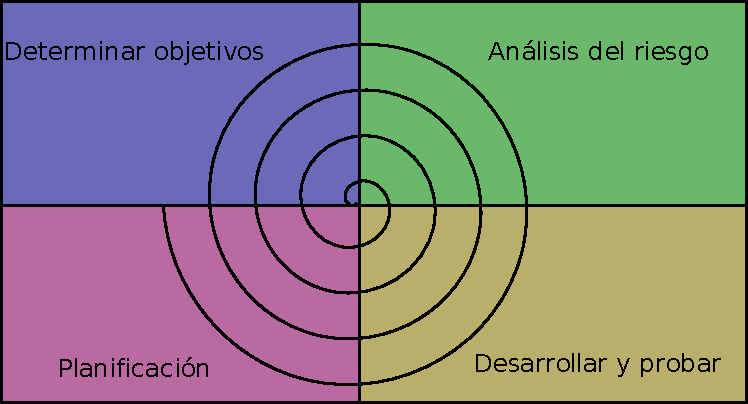
\includegraphics[scale=1]{modelo_espiral}
\end{center}
\end{figure}

Se ha elegido este método de desarrollo ya que se consigue un avance el proyecto siempre muy estable, pues toda funcionalidad añadida al software es probada y evaluada. De esta forma, aunque el proyecto no esté completo, siempre se tiene una parte funcional, y se va incrementando de forma que siempre disponemos de un producto mínimamente viable. 

\section{Gestión de recursos}

Los proyectos que se pueden realizar dependen en gran medida de los recursos que se pueden destinar a ellos. Se requieren unos elementos mínimos que son indispensables para poder llevarlo a cabo. Por ello, es muy importante contar con los recursos necesarios y gestionarlos de manera adecuada.

\subsection{Recursos humanos}

El proyecto consta de un equipo de 3 personas para llevarlo a cabo:

\begin{itemize}
\item Ana Buendía Ruiz-Azuaga, se encarga de:
	\begin{itemize}
	\item Planificación y análisis del proyecto.
	\item Búsqueda de bibliografía.
	\item Diseño e implementación del proyecto.
	\item Pruebas para el correcto funcionamiento del proyecto.
	\item Redacción de la documentación del proyecto.
	\end{itemize}
\item Tutores: Manuel Pegalajar Cuéllar y Teresa E. Pérez Fernández, encargados de:
	\begin{itemize}
	\item Idea original del proyecto.
	\item Proporcionar bibliografía.
	\item Guiar para la redacción de la memoria y documentación.
	\item Supervisar el desarrollo del proyecto.
	\end{itemize}
\end{itemize}

\subsection{Recursos hardware}

Todo el proyecto se va a desarrollar en un ordenador portátil con todo el software y dependencias necesarias. Las especificaciones del portátil son:

\begin{itemize}
\item \textbf{Modelo}: Acer Aspire E-5 574G.
\item \textbf{CPU}: Intel Core i5-6200U.
\item \textbf{RAM} 8GB RAM DDR3.
\item \textbf{Disco duro}: 1TB.
\item \textbf{Precio}: 600€.
\end{itemize}

\subsection{Recursos software}

El proyecto se ha llevado a cabo usando como sistema operativo Ubuntu 20.04 LTS, y se ha usado como lenguaje principal Python.

El software necesario para el proyecto es el siguiente:

\begin{itemize}
\item \textbf{Flask}. Flask es un microframework web en Python. Proporciona funcionalidad básica para, de forma sencilla, crear una aplicación web. Una posible alternativa habría sido Django, pero finalmente se ha optado por Flask debido a su simplicidad, legibilidad y que en este proyecto no se requieren muchas de las funcionalidades que Django ofrece integradas. La documentación de Flask puede verse aquí \cite{flask}.
\item \textbf{Dash}. Dash es un framework opensource basado en plotly.js y react.js que permite crear fácilmente aplicaciones basadas en datos. En este proyecto se ha usado principalmente por su capacidad de crear gráficas interactivas en tiempo real. La documentación del framework puede consultarse aquí \cite{dash}.
\item \textbf{Scipy}. Scipy es una librería de código abierto para python que proporciona algoritmos para optimización, integración, ecuaciones diferenciales y estadística, entre otros. Se ha usado principalmente para optimizar, integrar en los modelos continuos y realizar los ajustes. Para su utilización se ha consultado \cite{scipy}.
\item \textbf{VSCode}. Se ha usado VSCode como editor de texto, ya que proporciona una gran cantidad de plugins para cualquier lenguaje, así como integración con git.
\item \textbf{Draw.io}. Para la realización de diagramas de distintas clases, se ha usado el software de dibujo gratuito Draw.io.
\item \textbf{Docker}. Con el fin de simplificar el lanzamiento y ejecución de la aplicación web desarrollada se ha usado docker para virtualizar el entorno y evitar la necesidad de instalar en cualquier máquina el software necesario para ejecutarla. Durante el desarrollo, para facilitar la utilización de esta herramienta se ha consultado la documentación de docker \cite{docker}, usando docker compose, \cite{dockercompose}, para construir el contenedor y docker hub, \cite{dockerhub}, para la publicación del mismo.
\item \textbf{Git y Github}. Se ha empleado Git como controlador de versiones, integrado con Github. Puede consultarse más información sobre esta herramienta en \cite{git}.También se puede ver el desarrollo del proyecto en el \href{https://github.com/Mapachana/TFG}{repositorio de Github}\footnote{El enlace es \href{https://github.com/Mapachana/TFG}{https://github.com/Mapachana/TFG}}.
\item \textbf{Texmaker}. Para redactar la memoria, se ha usado el editor de LaTeX Texmaker.
\end{itemize}

Todo el software utilizado ha sido gratuito, por lo que no ha tenido coste alguno.

\subsection{Estimación del coste}

A partir de los recursos previamente listados, se va a realizar una aproximación del coste de la consecución del proyecto, considerando que la duración del mismo es de 9 meses.

Para los recursos humanos, dado que se considera que la alumna ha trabajado aproximadamente 450 horas de acuerdo a los $18$ créditos ECTS correspondientes asignados al TFG, y el gasto aproximado es 15€/h en calidad de alumna de prácticas, se tiene que el coste es de 6.750,00€.

A los tutores, dada su formación profesional se les supone un coste estimado de 50€/h, y aproximando que se dedican 3 horas semanales para la tutorización del proyecto, se tiene que el coste total tras los 9 meses es de 5.400,00€ por tutor.

Dado que el portátil empleado tiene una vida útil estimada de 5 años, le corresponde un coste de 120,00€ por amortización durante la realización del proyecto.

Finalmente, todo el software empleado es gratuito. El coste aproximado del proyecto aparece desglosado en la tabla \ref{tabla_pres}.

\begin{table}[!h]
\caption{Desglose de presupuesto del proyecto.}
\begin{center}
\begin{tabular}{|c c|} 
 \hline
 \textbf{Recursos humanos} & \textbf{Coste (€)} \\ 
 \hline\hline
 Alumna & 6.750,00 \\
 \hline
 Tutor 1 & 5.400,00 \\
 \hline 
 Tutor 2 & 5.400,00 \\
 \hline
 \textbf{Suma} & \textbf{17.550,00} \\
 \hline
 \textbf{Recursos hardware} & \textbf{Coste (€)} \\ 
 \hline\hline
 Ordenador portátil & 120,00 \\
 \hline
 \textbf{Suma} & \textbf{120,00} \\
 \hline 
 \textbf{Recursos software} & \textbf{Coste (€)} \\
 \hline
  Flask & 0,00 \\
  \hline
  Dash & 0,00 \\
  \hline 
  Scipy & 0,00 \\
  \hline 
  VSCode & 0,00 \\
  \hline
  TexMaker & 0,00 \\
  \hline 
  \textbf{Suma} & \textbf{0,00} \\ 
 \hline\hline
 \textbf{Suma total} & \textbf{17.670,00} \\
 \hline\hline
 \textbf{Gastos indirectos (18\%)} & \textbf{3.180,60} \\ 
 \hline\hline
 \textbf{Total} & \textbf{20.850,60} \\ 
 \hline\hline
 \textbf{IVA (21\%)} & \textbf{4.378,63} \\ % es .626 
 \hline\hline
 \textbf{Coste final} & \textbf{25.229,23} \\  % es .226
 \hline\hline

 \hline
\end{tabular}
\label{tabla_pres}
\end{center}
\end{table}

\section{Planificación temporal}

Para la realización del proyecto se han distinguido distintas etapas, y en cada una de ellas se ha implementado y trabajado sobre una funcionalidad concreta, de acuerdo al modelo en espiral. Las distintas partes del proyecto han sido:

\begin{itemize}
\item \textbf{T1. Estudio de bibliografía y estado actual de la epidemiología}. Se han consultado diversos libros, artículos y páginas de interés con el fin de comprender mejor y obtener los recursos necesarios para la realización de la parte teórica del proyecto. Además, se ha realizado una selección de los modelos a estudiar y tratar durante el desarrollo del mismo.
\item \textbf{T2. Especificación de requisitos}. En base a la información obtenida de la primera parte, en esta etapa se han especificado los requisitos que el software debe cumplir.
\item \textbf{T3. Diseño del sistema}. A partir de los requisitos especificados, se ha diseñado la arquitectura del sistema y cómo será la interfaz con la que van a interactuar los usuarios.
\item \textbf{T4. Marco teórico}. Se han indicado conceptos y modelos, así como estudiado las características de estos con el fin de desarrollar la teoría necesaria para trabajar con modelos epidemiológicos. Asimismo, se ha indicado el contexto en el que la epidemiología es de gran utilidad.
\item \textbf{T5. Implementación de los modelos discretos}. Se ha realizado la implementación de los modelos discretos SI, SIR y SIS, incluyendo gráficas interactivas de los mismos.
\item \textbf{T6. Implementación de los modelos continuos}. Se ha realizado la implementación de los modelos continuos SI, SIR y SIS, incluyendo gráficas interactivas de los mismos, al igual que información teórica.
\item \textbf{T7. Ajuste de datos a diversos modelos}. Se ha implementado una funcionalidad para realizar un ajuste de parámetros de acuerdo a un modelo a elegir, o el sistema puede determinar cuál es el modelo que minimiza el error para unos datos dados.
\item \textbf{T8. Documentación del proyecto}. Se ha llevado a cabo la documentación del proyecto durante todo su desarrollo.
\end{itemize}

Con el fin de ayudar a hacer más fácil la comprensión de cómo se ha distribuido el tiempo del proyecto, se ha realizado el diagrama \ref{fig: planificacion} en el que se puede ver cuánto tiempo se ha dedicado a cada etapa del desarrollo del proyecto durante los $9$ meses de duración del mismo.

\begin{figure}[!h]
\begin{center}
\caption{Planificación temporal de las etapas del proyecto.}
\label{fig: planificacion}
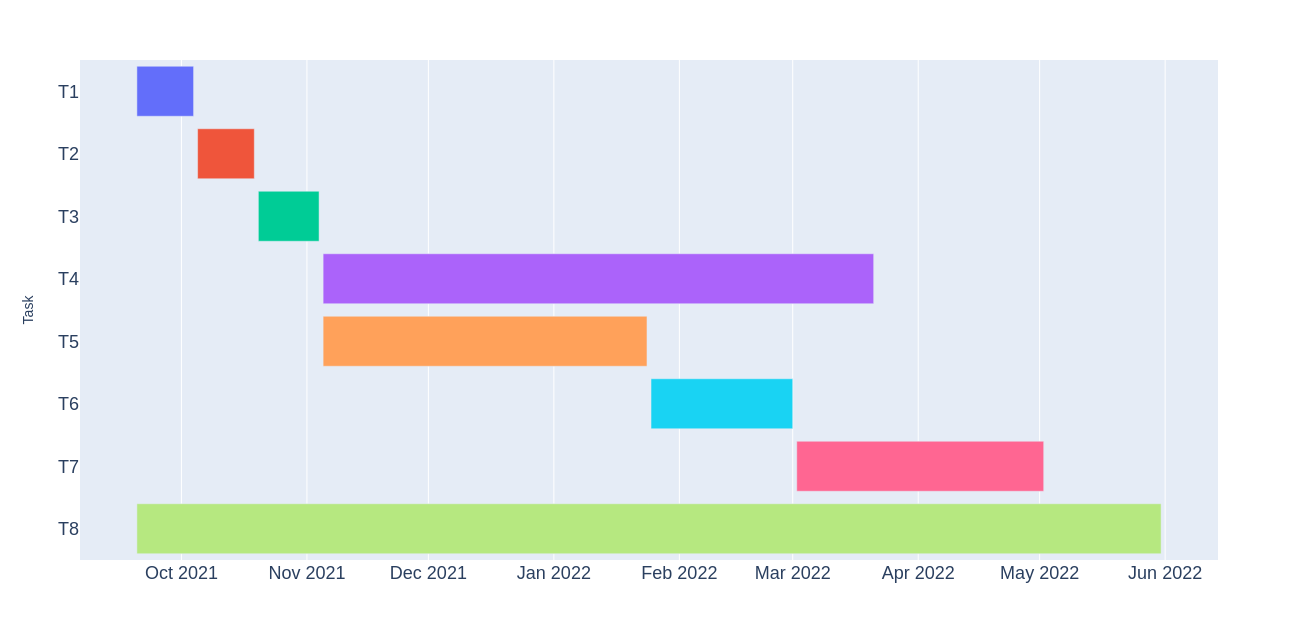
\includegraphics[scale=0.35]{planificacion}
\end{center}
\end{figure}


\section{Diagrama conceptual}

Para el modelado conceptual de la aplicación web, se ha optado por utilizar OOWS (Object-Oriented approach for Web Solutions modeling) \cite{pastorobject}, que usa modelado de objetos UML y modelos de navegación y presentación usando UML. Así, se expresan las características navegacionales de la aplicación web a la vez que se integra con las restantes vistas del esquema conceptual mediante una notación UML adaptada.

En la figura \ref{diag: modelo_concep}, se muestra el diagrama conceptual, construido mediante una estrategia top-down (de más general a menos):

\begin{figure}[!h]
\begin{center}
\caption{Modelo conceptual de la aplicación web.}
\label{diag: modelo_concep}
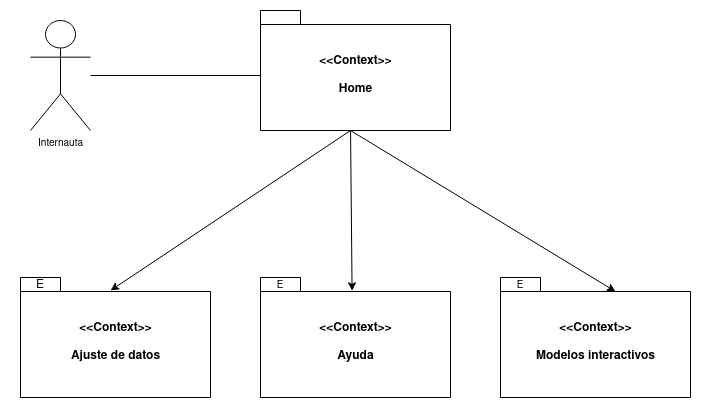
\includegraphics[scale=0.5]{modelo_conceptual-vista-paquetes.drawio}
\end{center}
\end{figure}

En la figura \ref{diag: modelo_concep_home} se muestra el detalle del contexto de \verb|Home|, en la figura \ref{diag: modelo_concep_modelos} se ve el detalle de \verb|Modelos Interactivos|, así como en \ref{diag: modelo_concep_ayuda} el de \verb|Ayuda| y en \ref{diag: modelo_concep_ajuste} el de \verb|Ajuste de datos|.

\begin{figure}[!h]
\begin{center}
\caption{Modelo conceptual del contexto de Inicio.}
\label{diag: modelo_concep_home}
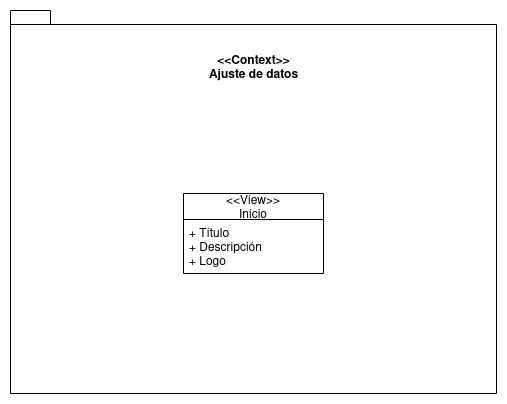
\includegraphics[scale=0.5]{modelo_conceptual-home.drawio}
\end{center}
\end{figure}

\begin{figure}[!h]
\begin{center}
\caption{Modelo conceptual del contexto de Modelos Interactivos.}
\label{diag: modelo_concep_modelos}
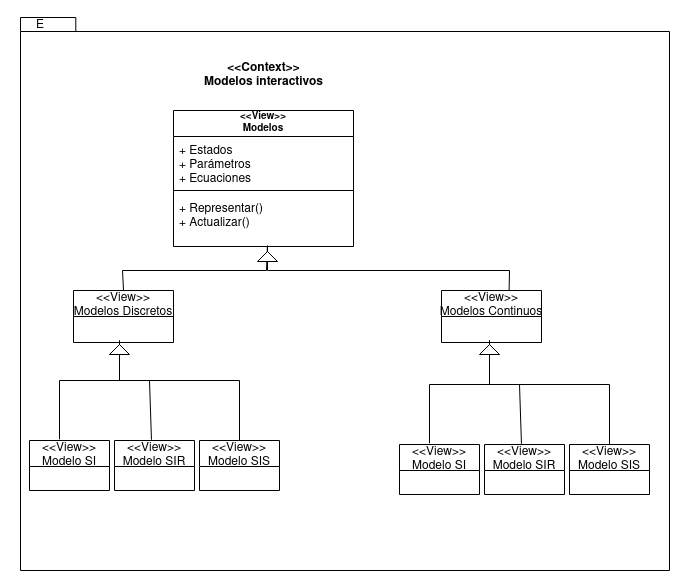
\includegraphics[scale=0.5]{modelo_conceptual-Modelos.drawio}
\end{center}
\end{figure}

\begin{figure}[!h]
\begin{center}
\caption{Modelo conceptual del contexto de Ayuda.}
\label{diag: modelo_concep_ayuda}
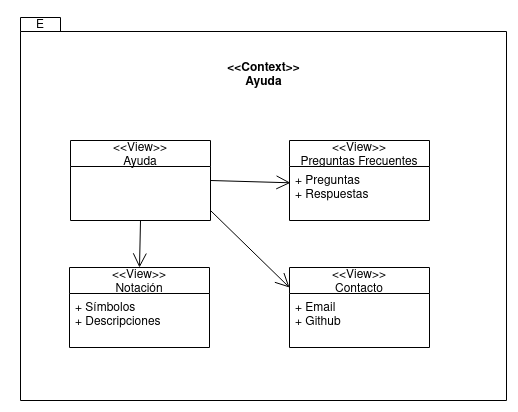
\includegraphics[scale=0.5]{modelo_conceptual-Ayuda.drawio}
\end{center}
\end{figure}

\begin{figure}[!h]
\begin{center}
\caption{Modelo conceptual del contexto de Ajuste de Datos.}
\label{diag: modelo_concep_ajuste}
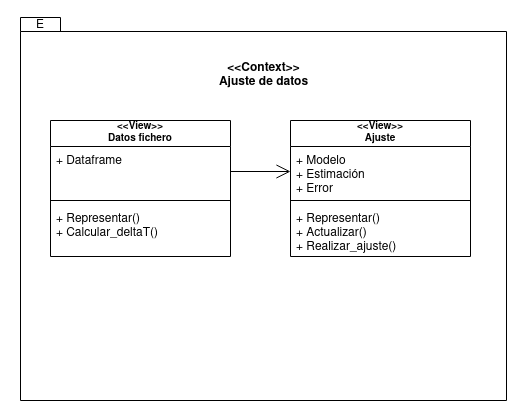
\includegraphics[scale=0.5]{modelo_conceptual-Ajuste.drawio}
\end{center}
\end{figure}





\section{Casos de uso}

A partir de los requisitos listados anteriormente, se obtienen los siguientes casos de uso:

\begin{itemize}
\item \textbf{CU-1}: Modificar parámetro de un modelo.
\item \textbf{CU-2}: Preprocesar entrada.
\item \textbf{CU-3}: Subir fichero de datos.
\item \textbf{CU-4}: Leer fichero de datos.
\item \textbf{CU-5}: Actualizar gráfica.
\item \textbf{CU-6}: Seleccionar modelo de ajuste.
\item \textbf{CU-7}: Realizar ajuste de datos.
\item \textbf{CU-8}: Descargar gráfica.
\end{itemize}

\subsection{Actores del sistema}

En este sistema solo tenemos un actor, que es el usuario que va a usar la página web. La información del usuario puede consultarse en el cuadro \ref{tab: actores}.

\begin{table}[!h]
\caption{Actores del sistema.}
\begin{tabular}{|c|c|c|c|c|c|c|c|}
\hline
 \rowcolor{azulillo} \textbf{Actor} & \multicolumn{6}{|c|}{Usuario} & {A-1} \\
\hline
 \cellcolor{azulillo} \textbf{Descripción}              & \multicolumn{7}{|c|}{Representa el usuario estándar que va a usar la página web.}           \\
\hline
 \cellcolor{azulillo} \textbf{Características}                 & \multicolumn{7}{|c|}{Interactúa con la aplicación web de forma directa.}             \\
\hline
 \cellcolor{azulillo} \textbf{Relaciones}         & \multicolumn{7}{|c|}{}             \\
\hline
\cellcolor{azulillo} \textbf{Referencias}        & \multicolumn{7}{|c|}{Interviene en los casos de uso CU-1, CU-3 y CU-6.}              \\
\hline
\cellcolor{azulillo} \textbf{Autor}                &   Ana  & \multicolumn{2}{|c|}{\cellcolor{azulillo} \textbf{Fecha}} &  25/04/22   & \multicolumn{2}{|c|}{\cellcolor{azulillo} \textbf{Versión}} & 1.0  \\
\hline
\end{tabular}
\label{tab: actores}
\end{table}

\subsection{Diagrama de casos de uso}

Se incluye también el diagrama de los casos de uso, con el fin de ilustrar todos los posibles casos de uso, así como sus relaciones entre ellos. El diagrama resultante puede verse en la figura \ref{diag: casos_uso}.

\begin{figure}[!h]
\begin{center}
\caption{Diagrama de casos de uso}
\label{diag: casos_uso}
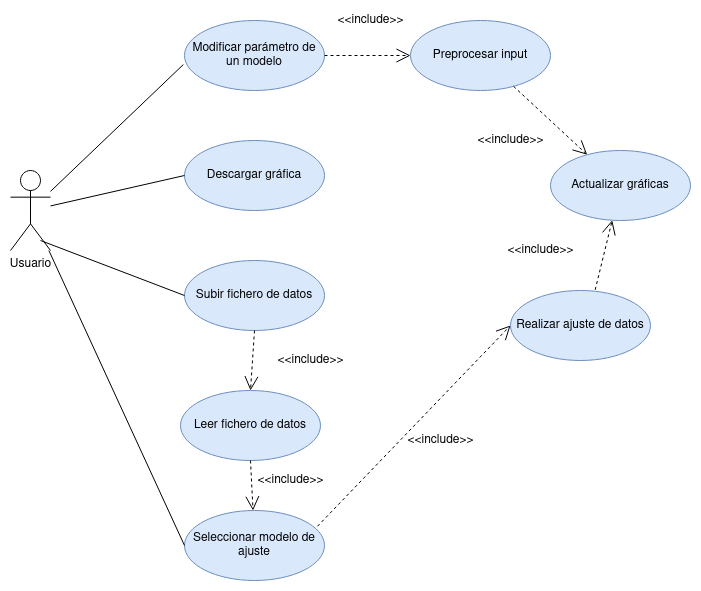
\includegraphics[scale=0.5]{casos_de_uso.drawio}
\end{center}
\end{figure}




\subsection{Plantillas de casos de uso}

Para cada uno de los casos de uso mencionados se ha rellenado una plantilla descriptiva con información necesaria del desarrollo de estos. En esta plantilla se detallan las condiciones que deben cumplirse antes y después del caso de uso, así como su propósito, su funcionamiento y su curso, pudiendo ser este un curso normal (o esperado) o alterno (menos frecuente).

\clearpage

\begin{table}[!h]
\begin{tabularx}{\textwidth}{|Y|Y|Y|Y|Y|Y|Y|Y|Y|}
\hline
\rowcolor{azulillo} \multicolumn{2}{|c|}{\textbf{Caso de uso}} & \multicolumn{5}{|c|}{Modificar parámetro de un modelo} & \multicolumn{2}{|c|}{CU-1} \\
\hline
\multicolumn{2}{|c|}{\cellcolor{azulillo} \textbf{Actores}}              & \multicolumn{7}{|c|}{Usuario}           \\
\hline
\multicolumn{2}{|c|}{\cellcolor{azulillo} \textbf{Tipo}}                 & \multicolumn{7}{|c|}{Esencial}             \\
\hline
\multicolumn{2}{|c|}{\cellcolor{azulillo} \textbf{Referencias}}          & \multicolumn{2}{|c|}{RF1}           & \multicolumn{5}{|c|}{CU-2, CU-5}\\
\hline
\multicolumn{2}{|c|}{\cellcolor{azulillo} \textbf{Precondición}}         & \multicolumn{7}{|c|}{Se debe estar trabajando con un modelo.}             \\
\hline
\multicolumn{2}{|c|}{\cellcolor{azulillo} \textbf{Postcondición}}        & \multicolumn{7}{|c|}{Se debe preprocesar la entrada.}              \\
\hline
\multicolumn{2}{|c|}{\cellcolor{azulillo} \textbf{Autor}}               &   Ana  & \multicolumn{2}{|c|}{\cellcolor{azulillo} \textbf{Fecha}} &  25/04/22   & \multicolumn{2}{|c|}{\cellcolor{azulillo} \textbf{Versión}} & 1.0  \\
\hline
\end{tabularx}
\end{table}

\begin{table}[!h]
\begin{tabularx}{\textwidth}{|Y|}
\hline
\cellcolor{azulillo} \textbf{Propósito} \\
\hline
Modificar uno de los parámetros disponibles del modelo para ver cómo afecta al  comportamiento del mismo.   \\
\hline
\end{tabularx}
\end{table}

\begin{table}[!h]
\begin{tabularx}{\textwidth}{|Y|}
\hline
\cellcolor{azulillo} \textbf{Resumen}  \\
\hline
Se modifica uno de los parámetros posibles del modelo, modificando así su comportamiento y visualizando la nueva gráfica resultante.   \\
\hline
\end{tabularx}
\end{table}

\begin{table}[!h]
\begin{tabularx}{\textwidth}{|c|Y|c|Y|}
\hline
\multicolumn{4}{|c|}{ \cellcolor{azulillo}Curso normal} \\
\hline
      1.        &  El usuario modifica un parámetro     &              &              \\
\hline
              &               &       2.       &      Incluir CU-2         \\
\hline
              &               &       3.       &      Incluir CU-5        \\

\hline
\end{tabularx}
\end{table}

\begin{table}[!h]
\begin{tabularx}{\textwidth}{|c|Y|}
\hline
\multicolumn{2}{|c|}{\cellcolor{azulillo} \textbf{Cursos alternos}} \\
\hline
       2a.       &      El formato no es correcto, se asigna un valor por defecto        \\
\hline
       3a.       &      Incluir CU-5        \\
\hline
\end{tabularx}
\end{table}

\begin{table}[!h]
\begin{tabularx}{\textwidth}{|Y|Y|Y|Y|}
\hline
\multicolumn{4}{|c|}{\cellcolor{azulillo} \textbf{Otros datos}} \\
\hline
 \cellcolor{azulillo} \textbf{Frecuencia esperada}             &     Alta          &    \cellcolor{azulillo} \textbf{Rendimiento}          &      Alto        \\
\hline
 \cellcolor{azulillo} \textbf{Importancia}             &      Vital         &     \cellcolor{azulillo} \textbf{Urgencia}         &      Alta        \\
\hline
 \cellcolor{azulillo} \textbf{Estado}             &      Finalizado         &    \cellcolor{azulillo} \textbf{Estabilidad}          &     Alta         \\
\hline
 \cellcolor{azulillo} \textbf{Comentarios}        &  \multicolumn{3}{|c|}{-} \\
\hline
\end{tabularx}
\end{table}





\clearpage

\begin{table}[!h]
\begin{tabularx}{\textwidth}{|Y|Y|Y|Y|Y|Y|Y|Y|Y|}
\hline
\rowcolor{azulillo} \multicolumn{2}{|c|}{\textbf{Caso de uso}} & \multicolumn{5}{|c|}{Preprocesar entrada} & \multicolumn{2}{|c|}{CU-2} \\
\hline
\multicolumn{2}{|c|}{\cellcolor{azulillo} \textbf{Actores} }             & \multicolumn{7}{|c|}{(Sistema)}           \\
\hline
\multicolumn{2}{|c|}{\cellcolor{azulillo} \textbf{Tipo}  }               & \multicolumn{7}{|c|}{Esencial}             \\
\hline
\multicolumn{2}{|c|}{\cellcolor{azulillo} \textbf{Referencias}  }        & \multicolumn{2}{|c|}{RF-1}           & \multicolumn{5}{|c|}{CU-1}\\
\hline
\multicolumn{2}{|c|}{\cellcolor{azulillo} \textbf{Precondición} }        & \multicolumn{7}{|c|}{Se debe haber modificado un parámetro del modelo.}             \\
\hline
\multicolumn{2}{|c|}{\cellcolor{azulillo} \textbf{Postcondición} }       & \multicolumn{7}{|c|}{Se debe actualizar la gráfica. }              \\
\hline
\multicolumn{2}{|c|}{\cellcolor{azulillo} \textbf{Autor}   }             &   Ana   & \multicolumn{2}{|c|}{\cellcolor{azulillo} \textbf{Fecha}} &  25/04/22   & \multicolumn{2}{|c|}{\cellcolor{azulillo} \textbf{Versión}} & 1.0  \\
\hline
\end{tabularx}
\end{table}

\begin{table}[!h]
\begin{tabularx}{\textwidth}{|Y|}
\hline
\cellcolor{azulillo} \textbf{Propósito} \\
\hline
Asegurar el correcto formato y validez del valor introducido. \\
\hline
\end{tabularx}
\end{table}

\begin{table}[!h]
\begin{tabularx}{\textwidth}{|Y|}
\hline
\cellcolor{azulillo} \textbf{Resumen}  \\
\hline
 Se comprueba la validez y formato del valor introducido para asegurar el correcto funcionamiento del modelo.  \\
\hline
\end{tabularx}
\end{table}

\begin{table}[!h]
\begin{tabularx}{\textwidth}{|c|Y|c|Y|}
\hline
\multicolumn{4}{|c|}{\cellcolor{azulillo} \textbf{Curso normal}} \\
\hline
              &               &      1.        &    Se comprueba el tipo de valor (float o entero).         \\
\hline
              &               &      2.        &    Se  comprueba el rango de validez de los valors de cada parámetro.         \\
\hline
              &               &      3.        &    Se comprueba que la población sea constante.          \\
\hline
\end{tabularx}
\end{table}

\begin{table}[!h]
\begin{tabularx}{\textwidth}{|c|Y|}
\hline
\multicolumn{2}{|c|}{\cellcolor{azulillo} \textbf{Cursos alternos}} \\
\hline
        1a       &     Si el valor no es de un tipo válido se sustituye por $0$. \\
\hline
        2b.      &     Si el valor no está en el rango se sustituye por $0$.         \\
\hline

\end{tabularx}
\end{table}

\begin{table}[!h]
\begin{tabularx}{\textwidth}{|Y|Y|Y|Y|}
\hline
\multicolumn{4}{|c|}{\cellcolor{azulillo} \textbf{Otros datos}} \\
\hline
 \cellcolor{azulillo} \textbf{Frecuencia esperada}             &      Alta         &    \cellcolor{azulillo} \textbf{Rendimiento}          &      Alto        \\
\hline
 \cellcolor{azulillo} \textbf{Importancia}             &      Vital         &     \cellcolor{azulillo} \textbf{Urgencia}         &      Alta        \\
\hline
 \cellcolor{azulillo} \textbf{Estado}             &       Finalizado        &    \cellcolor{azulillo} \textbf{Estabilidad}          &    Alta          \\
\hline
 \cellcolor{azulillo} \textbf{Comentarios}        &  \multicolumn{3}{|c|}{-} \\
\hline
\end{tabularx}
\end{table}






\clearpage

\begin{table}[!h]
\begin{tabularx}{\textwidth}{|Y|Y|Y|Y|Y|Y|Y|Y|Y|}
\hline
\rowcolor{azulillo} \multicolumn{2}{|c|}{\textbf{Caso de uso}} & \multicolumn{5}{|c|}{Subir fichero de datos} & \multicolumn{2}{|c|}{CU-3} \\
\hline
\multicolumn{2}{|c|}{\cellcolor{azulillo} \textbf{Actores}}              & \multicolumn{7}{|c|}{Usuario}           \\
\hline
\multicolumn{2}{|c|}{\cellcolor{azulillo} \textbf{Tipo} }                & \multicolumn{7}{|c|}{Esencial}             \\
\hline
\multicolumn{2}{|c|}{\cellcolor{azulillo} \textbf{Referencias}}          & \multicolumn{2}{|c|}{RF4}           & \multicolumn{5}{|c|}{CU-4, CU-5, CU-6, CU-7}\\
\hline
\multicolumn{2}{|c|}{\cellcolor{azulillo} \textbf{Precondición}}         & \multicolumn{7}{|c|}{-}             \\
\hline
\multicolumn{2}{|c|}{\cellcolor{azulillo} \textbf{Postcondición}}        & \multicolumn{7}{|c|}{-}              \\
\hline
\multicolumn{2}{|c|}{\cellcolor{azulillo} \textbf{Autor}  }              &   Ana  & \multicolumn{2}{|c|}{\cellcolor{azulillo} \textbf{Fecha}} &  25/04/22   & \multicolumn{2}{|c|}{\cellcolor{azulillo} \textbf{Versión}} & 1.0  \\
\hline
\end{tabularx}
\end{table}

\begin{table}[!h]
\begin{tabularx}{\textwidth}{|Y|}
\hline
\cellcolor{azulillo} \textbf{Propósito} \\
\hline
El usuario debe poder subir un fichero de datos para trabajar sobre él.  \\
\hline
\end{tabularx}
\end{table}

\begin{table}[!h]
\begin{tabularx}{\textwidth}{|Y|}
\hline
\cellcolor{azulillo} \textbf{Resumen}  \\
\hline
El usuario sube un fichero de datos.    \\
\hline
\end{tabularx}
\end{table}

\begin{table}[!h]
\begin{tabularx}{\textwidth}{|c|Y|c|Y|}
\hline
\multicolumn{4}{|c|}{\cellcolor{azulillo} \textbf{Curso normal}} \\
\hline
      1.        &      El usuario selecciona un fichero de datos.         &              &              \\
\hline
              &               &      2.        &    El sistema sube el fichero de datos seleccionado.          \\
\hline
\end{tabularx}
\end{table}

\begin{table}[!h]
\begin{tabularx}{\textwidth}{|c|Y|}
\hline
\multicolumn{2}{|c|}{\cellcolor{azulillo} \textbf{Cursos alternos}} \\
\hline
      2a.        &    El fichero no tiene formato correcto, por lo que no se deja seleccionarlo.          \\
\hline
\end{tabularx}
\end{table}

\begin{table}[!h]
\begin{tabularx}{\textwidth}{|Y|Y|Y|Y|}
\hline
\multicolumn{4}{|c|}{\cellcolor{azulillo} \textbf{Otros datos}} \\
\hline
 \cellcolor{azulillo} \textbf{Frecuencia esperada}             &     Alta          &    \cellcolor{azulillo} \textbf{Rendimiento}          &      Alto        \\
\hline
 \cellcolor{azulillo} \textbf{Importancia}             &      Vital         &     \cellcolor{azulillo} \textbf{Urgencia}         &      Alta        \\
\hline
 \cellcolor{azulillo} \textbf{Estado}             &      Finalizado         &    \cellcolor{azulillo} \textbf{Estabilidad}          &     Alta         \\
\hline
 \cellcolor{azulillo} \textbf{Comentarios}        &  \multicolumn{3}{|c|}{-} \\
\hline
\end{tabularx}
\end{table}




\clearpage

\begin{table}[!h]
\begin{tabularx}{\textwidth}{|Y|Y|Y|Y|Y|Y|Y|Y|Y|}
\hline
\rowcolor{azulillo} \multicolumn{2}{|c|}{\textbf{Caso de uso}} & \multicolumn{5}{|c|}{Leer fichero de datos} & \multicolumn{2}{|c|}{CU-4} \\
\hline
\multicolumn{2}{|c|}{\cellcolor{azulillo} \textbf{Actores}}              & \multicolumn{7}{|c|}{(Sistema)}           \\
\hline
\multicolumn{2}{|c|}{\cellcolor{azulillo} \textbf{Tipo}}                 & \multicolumn{7}{|c|}{Esencial}             \\
\hline
\multicolumn{2}{|c|}{\cellcolor{azulillo} \textbf{Referencias}}          & \multicolumn{2}{|c|}{RF4}           & \multicolumn{5}{|c|}{CU-3, CU-7}\\
\hline
\multicolumn{2}{|c|}{\cellcolor{azulillo} \textbf{Precondición}}         & \multicolumn{7}{|c|}{Se debe haber subido el fichero a leer.}             \\
\hline
\multicolumn{2}{|c|}{\cellcolor{azulillo} \textbf{Postcondición}}        & \multicolumn{7}{|c|}{Se debe actualizar la gráfica.}              \\
\hline
\multicolumn{2}{|c|}{\cellcolor{azulillo} \textbf{Autor} }               &   Ana   & \multicolumn{2}{|c|}{\cellcolor{azulillo} \textbf{Fecha}} &  25/04/22   & \multicolumn{2}{|c|}{\cellcolor{azulillo} \textbf{Versión}} & 1.0  \\
\hline
\end{tabularx}
\end{table}

\begin{table}[!h]
\begin{tabularx}{\textwidth}{|Y|}
\hline
\cellcolor{azulillo} \textbf{Propósito} \\
\hline
 Leer el fichero para poder trabajar con los datos que contiene.                  \\
\hline
\end{tabularx}
\end{table}

\begin{table}[!h]
\begin{tabularx}{\textwidth}{|Y|}
\hline
\cellcolor{azulillo} \textbf{Resumen}  \\
\hline
 Se lee el fichero de datos cargando estos en memoria.                  \\
\hline
\end{tabularx}
\end{table}

\begin{table}[!h]
\begin{tabularx}{\textwidth}{|c|Y|c|Y|}
\hline
\multicolumn{4}{|c|}{\cellcolor{azulillo} \textbf{Curso normal}} \\
\hline
              &               &      1.        &     Se abre el fichero         \\
\hline
              &               &      2.        &     Se lee el fichero         \\
\hline
\end{tabularx}
\end{table}

\begin{table}[!h]
\begin{tabularx}{\textwidth}{|c|Y|}
\hline
\multicolumn{2}{|c|}{\cellcolor{azulillo} \textbf{Cursos alternos}} \\
\hline
    2a.          &      Si el formato del fichero no es el esperado, se muestra un error.        \\
\hline
\end{tabularx}
\end{table}

\begin{table}[!h]
\begin{tabularx}{\textwidth}{|Y|Y|Y|Y|}
\hline
\multicolumn{4}{|c|}{\cellcolor{azulillo} \textbf{Otros datos}} \\
\hline
 \cellcolor{azulillo} \textbf{Frecuencia esperada}             &      Alta         &    \cellcolor{azulillo} \textbf{Rendimiento}          &      Alto        \\
\hline
 \cellcolor{azulillo} \textbf{Importancia}             &       Vital        &     \cellcolor{azulillo} \textbf{Urgencia}         &      Alta        \\
\hline
 \cellcolor{azulillo} \textbf{Estado}             &       Finalizado        &    \cellcolor{azulillo} \textbf{Estabilidad}          &      Alta        \\
\hline
 \cellcolor{azulillo} \textbf{Comentarios}        &  \multicolumn{3}{|c|}{-} \\
\hline
\end{tabularx}
\end{table}





\clearpage

\begin{table}[!h]
\begin{tabularx}{\textwidth}{|Y|Y|Y|Y|Y|Y|Y|Y|Y|}
\hline
\rowcolor{azulillo} \multicolumn{2}{|c|}{\textbf{Caso de uso}} & \multicolumn{5}{|c|}{Actualizar gráficas} & \multicolumn{2}{|c|}{CU-5} \\
\hline
\multicolumn{2}{|c|}{\cellcolor{azulillo} \textbf{Actores} }             & \multicolumn{7}{|c|}{(Sistema)}           \\
\hline
\multicolumn{2}{|c|}{\cellcolor{azulillo} \textbf{Tipo}  }               & \multicolumn{7}{|c|}{Esencial}             \\
\hline
\multicolumn{2}{|c|}{\cellcolor{azulillo} \textbf{Referencias} }         & \multicolumn{2}{|c|}{RF1, RF2, RF5}           & \multicolumn{5}{|c|}{CU-1, CU-6}\\
\hline
\multicolumn{2}{|c|}{\cellcolor{azulillo} \textbf{Precondición}}         & \multicolumn{7}{|c|}{Se ha modificado un parámetro o ajuste seleccionado.}             \\
\hline
\multicolumn{2}{|c|}{\cellcolor{azulillo} \textbf{Postcondición}  }      & \multicolumn{7}{|c|}{La gráfica se ha actualizado.}              \\
\hline
\multicolumn{2}{|c|}{\cellcolor{azulillo} \textbf{Autor}   }             &   Ana   & \multicolumn{2}{|c|}{\cellcolor{azulillo} \textbf{Fecha}} &  25/04/22   & \multicolumn{2}{|c|}{\cellcolor{azulillo} \textbf{Versión}} & 1.0  \\
\hline
\end{tabularx}
\end{table}

\begin{table}[!h]
\begin{tabularx}{\textwidth}{|Y|}
\hline
\cellcolor{azulillo} \textbf{Propósito} \\
\hline
Actualizar la gráfica para tener la visualización de los datos de acuerdo a las opciones indicadas.   \\
\hline
\end{tabularx}
\end{table}

\begin{table}[!h]
\begin{tabularx}{\textwidth}{|Y|}
\hline
\cellcolor{azulillo} \textbf{Resumen}  \\
\hline
Actualizar la gráfica cuando el usuario realiza una modificación de parámetros o del modelo con el que realizar el ajuste.  \\
\hline
\end{tabularx}
\end{table}

\begin{table}[!h]
\begin{tabularx}{\textwidth}{|c|Y|c|Y|}
\hline
\multicolumn{4}{|c|}{\cellcolor{azulillo} \textbf{Curso normal}} \\
\hline
              &               &      1.        &     Incluir CU-4         \\
\hline
              &               &      2.        &     Representar los datos con el nuevo parámetro.         \\
\hline
\end{tabularx}
\end{table}

\begin{table}[!h]
\begin{tabularx}{\textwidth}{|c|Y|}
\hline
\multicolumn{2}{|c|}{\cellcolor{azulillo} \textbf{Cursos alternos}} \\
\hline
      2a.        &     Si se ha cambiado el modelo con el que realizar el ajuste, incluir CU-7.         \\
\hline
      3a.        &     Representar los datos con el nuevo ajuste.         \\
\hline
\end{tabularx}
\end{table}

\begin{table}[!h]
\begin{tabularx}{\textwidth}{|Y|Y|Y|Y|}
\hline
\multicolumn{4}{|c|}{\cellcolor{azulillo} \textbf{Otros datos}} \\
\hline
 \cellcolor{azulillo} \textbf{Frecuencia esperada}             &     Alta         &    \cellcolor{azulillo} \textbf{Rendimiento}          &      Medio        \\
\hline
 \cellcolor{azulillo} \textbf{Importancia}             &      Vital         &     \cellcolor{azulillo} \textbf{Urgencia}         &     Alta         \\
\hline
 \cellcolor{azulillo} \textbf{Estado}             &       Finalizado        &    \cellcolor{azulillo} \textbf{Estabilidad}          &     Alta         \\
\hline
 \cellcolor{azulillo} \textbf{Comentarios}        &  \multicolumn{3}{|c|}{-} \\
\hline
\end{tabularx}
\end{table}




\clearpage

\begin{table}[!h]
\begin{tabularx}{\textwidth}{|Y|Y|Y|Y|Y|Y|Y|Y|Y|}
\hline
\rowcolor{azulillo} \multicolumn{2}{|c|}{\textbf{Caso de uso}} & \multicolumn{5}{|c|}{Seleccionar modelo de ajuste} & \multicolumn{2}{|c|}{CU-6} \\
\hline
\multicolumn{2}{|c|}{\cellcolor{azulillo} \textbf{Actores}}              & \multicolumn{7}{|c|}{Usuario}           \\
\hline
\multicolumn{2}{|c|}{\cellcolor{azulillo} \textbf{Tipo}}                 & \multicolumn{7}{|c|}{Esencial}             \\
\hline
\multicolumn{2}{|c|}{\cellcolor{azulillo} \textbf{Referencias}}          & \multicolumn{2}{|c|}{RF2}           & \multicolumn{5}{|c|}{CU-5, CU-7}\\
\hline
\multicolumn{2}{|c|}{\cellcolor{azulillo} \textbf{Precondición} }        & \multicolumn{7}{|c|}{Se debe tener leído un fichero de datos.}             \\
\hline
\multicolumn{2}{|c|}{\cellcolor{azulillo} \textbf{Postcondición}}        & \multicolumn{7}{|c|}{Se debe realizar el ajuste con el nuevo modelo elegido.}              \\
\hline
\multicolumn{2}{|c|}{\cellcolor{azulillo} \textbf{Autor}}                &   Ana   & \multicolumn{2}{|c|}{\cellcolor{azulillo} \textbf{Fecha}} &  25/04/22   & \multicolumn{2}{|c|}{\cellcolor{azulillo} \textbf{Versión}} & 1.0  \\
\hline
\end{tabularx}
\end{table}

\begin{table}[!h]
\begin{tabularx}{\textwidth}{|Y|}
\hline
\cellcolor{azulillo} \textbf{Propósito} \\
\hline
Poder elegir el modelo con el que realizar el ajuste de los datos.  \\
\hline
\end{tabularx}
\end{table}

\begin{table}[!h]
\begin{tabularx}{\textwidth}{|Y|}
\hline
\cellcolor{azulillo} \textbf{Resumen}  \\
\hline
Seleccionar el modelo a partir del cuál se va a realizar el ajuste.  \\
\hline
\end{tabularx}
\end{table}

\begin{table}[!h]
\begin{tabularx}{\textwidth}{|c|Y|c|Y|}
\hline
\multicolumn{4}{|c|}{\cellcolor{azulillo} \textbf{Curso normal}} \\
\hline
      1.        &     El usuario selecciona un modelo         &              &              \\
\hline
              &               &      2.        &      Incluir CU-7        \\
\hline
              &               &      3.        &      Incluir CU-5        \\
\hline
\end{tabularx}
\end{table}

\begin{table}[!h]
\begin{tabularx}{\textwidth}{|c|Y|}
\hline
\multicolumn{2}{|c|}{\cellcolor{azulillo} \textbf{Cursos alternos}} \\
\hline
              &       -       \\
\hline
\end{tabularx}
\end{table}

\begin{table}[!h]
\begin{tabularx}{\textwidth}{|Y|Y|Y|Y|}
\hline
\multicolumn{4}{|c|}{\cellcolor{azulillo} \textbf{Otros datos}} \\
\hline
 \cellcolor{azulillo} \textbf{Frecuencia esperada}             &       Alta        &    \cellcolor{azulillo} \textbf{Rendimiento}          &       Alto       \\
\hline
 \cellcolor{azulillo} \textbf{Importancia}             &      Alta         &     \cellcolor{azulillo} \textbf{Urgencia}         &       Alta       \\
\hline
 \cellcolor{azulillo} \textbf{Estado}             &      Finalizado         &    \cellcolor{azulillo} \textbf{Estabilidad}          &      Alta        \\
\hline
 \cellcolor{azulillo} \textbf{Comentarios}        &  \multicolumn{3}{|c|}{-} \\
\hline
\end{tabularx}
\end{table}





\clearpage

\begin{table}[!h]
\begin{tabularx}{\textwidth}{|Y|Y|Y|Y|Y|Y|Y|Y|Y|}
\hline
\rowcolor{azulillo} \multicolumn{2}{|c|}{\textbf{Caso de uso}} & \multicolumn{5}{|c|}{Realizar ajuste de datos} & \multicolumn{2}{|c|}{CU-7} \\
\hline
\multicolumn{2}{|c|}{\cellcolor{azulillo} \textbf{Actores} }             & \multicolumn{7}{|c|}{(Sistema)}           \\
\hline
\multicolumn{2}{|c|}{\cellcolor{azulillo} \textbf{Tipo} }                & \multicolumn{7}{|c|}{Esencial}             \\
\hline
\multicolumn{2}{|c|}{\cellcolor{azulillo} \textbf{Referencias} }         & \multicolumn{2}{|c|}{RF6, RF7}           & \multicolumn{5}{|c|}{CU-3, CU-4, CU-5, CU-6}\\
\hline
\multicolumn{2}{|c|}{\cellcolor{azulillo} \textbf{Precondición}}         & \multicolumn{7}{|c|}{Se debe haber leído un fichero y seleccionado un modelo.}             \\
\hline
\multicolumn{2}{|c|}{\cellcolor{azulillo} \textbf{Postcondición}}        & \multicolumn{7}{|c|}{Actualizar las gráficas}              \\
\hline
\multicolumn{2}{|c|}{\cellcolor{azulillo} \textbf{Autor} }               &   Ana   & \multicolumn{2}{|c|}{\cellcolor{azulillo} \textbf{Fecha}} &  25/04/22   & \multicolumn{2}{|c|}{\cellcolor{azulillo} \textbf{Versión}} & 1.0  \\
\hline
\end{tabularx}
\end{table}

\begin{table}[!h]
\begin{tabularx}{\textwidth}{|Y|}
\hline
\cellcolor{azulillo} \textbf{Propósito} \\
\hline
Obtener una estimación de los parámetros y los errores correspondientes de acuerdo al modelo seleccionado. \\
\hline
\end{tabularx}
\end{table}

\begin{table}[!h]
\begin{tabularx}{\textwidth}{|Y|}
\hline
\cellcolor{azulillo} \textbf{Resumen}  \\
\hline
Se realiza el ajuste de un modelo elegido a los datos leídos. \\
\hline
\end{tabularx}
\end{table}

\begin{table}[!h]
\begin{tabularx}{\textwidth}{|c|Y|c|Y|}
\hline
\multicolumn{4}{|c|}{\cellcolor{azulillo} \textbf{Curso normal}} \\
\hline
     1.         &     Incluir CU-6           &              &              \\
\hline
              &               &    2.          &     Estimar parámetros         \\
\hline
              &               &    3.          &     Calcular errores         \\
\hline
              &               &    4.          &     Incluir CU-5            \\
\hline
\end{tabularx}
\end{table}

\begin{table}[!h]
\begin{tabularx}{\textwidth}{|c|Y|}
\hline
\multicolumn{2}{|c|}{\cellcolor{azulillo} \textbf{Cursos alternos}} \\
\hline
     2a.         &    Si se debe elegir el mejor modelo, se calculan los parámetros para todos los modelos          \\
\hline
     3a.         &    Se calculan los errores para todos los modelos          \\
\hline
     4a.         &    Se elige el mejor modelo de acuerdo a un criterio sobre los errores          \\
\hline
\end{tabularx}
\end{table}

\begin{table}[!h]
\begin{tabularx}{\textwidth}{|Y|Y|Y|Y|}
\hline
\multicolumn{4}{|c|}{\cellcolor{azulillo} \textbf{Otros datos}} \\
\hline
 \cellcolor{azulillo} \textbf{Frecuencia esperada}             &      Alta         &    \cellcolor{azulillo} \textbf{Rendimiento}          &      Alto        \\
\hline
 \cellcolor{azulillo} \textbf{Importancia}             &      Vital         &     \cellcolor{azulillo} \textbf{Urgencia}         &      Alta        \\
\hline
 \cellcolor{azulillo} \textbf{Estado}             &       Finalizado        &    \cellcolor{azulillo} \textbf{Estabilidad}          &     Alta         \\
\hline
\cellcolor{azulillo} \textbf{Comentarios}        &  \multicolumn{3}{|c|}{-} \\
\hline
\end{tabularx}
\end{table}



\clearpage

\begin{table}[!h]
\begin{tabularx}{\textwidth}{|Y|Y|Y|Y|Y|Y|Y|Y|Y|}
\hline
\rowcolor{azulillo} \multicolumn{2}{|c|}{\textbf{Caso de uso}} & \multicolumn{5}{|c|}{Descargar gráfica} & \multicolumn{2}{|c|}{CU-8} \\
\hline
\multicolumn{2}{|c|}{\cellcolor{azulillo} \textbf{Actores} }             & \multicolumn{7}{|c|}{Usuario}           \\
\hline
\multicolumn{2}{|c|}{\cellcolor{azulillo} \textbf{Tipo}}                 & \multicolumn{7}{|c|}{Secundario}             \\
\hline
\multicolumn{2}{|c|}{\cellcolor{azulillo} \textbf{Referencias}}          & \multicolumn{2}{|c|}{RF3}           & \multicolumn{5}{|c|}{}\\
\hline
\multicolumn{2}{|c|}{\cellcolor{azulillo} \textbf{Precondición} }        & \multicolumn{7}{|c|}{-}             \\
\hline
\multicolumn{2}{|c|}{\cellcolor{azulillo} \textbf{Postcondición}}        & \multicolumn{7}{|c|}{-}              \\
\hline
\multicolumn{2}{|c|}{\cellcolor{azulillo} \textbf{Autor} }               &   Ana   & \multicolumn{2}{|c|}{\cellcolor{azulillo} \textbf{Fecha}} &  25/04/22   & \multicolumn{2}{|c|}{\cellcolor{azulillo} \textbf{Versión}} & 1.0  \\
\hline
\end{tabularx}
\end{table}

\begin{table}[!h]
\begin{tabularx}{\textwidth}{|Y|}
\hline
\cellcolor{azulillo} \textbf{Propósito} \\
\hline
Descargar una gráfica generada por la aplicación web. \\
\hline
\end{tabularx}
\end{table}

\begin{table}[!h]
\begin{tabularx}{\textwidth}{|Y|}
\hline
\cellcolor{azulillo} \textbf{Resumen}  \\
\hline
Se descarga la imagen de una gráfica generada. \\
\hline
\end{tabularx}
\end{table}

\begin{table}[!h]
\begin{tabularx}{\textwidth}{|c|Y|c|Y|}
\hline
\multicolumn{4}{|c|}{\cellcolor{azulillo} \textbf{Curso normal}} \\
\hline
     1.         &     Pulsa en descargar imagen           &              &              \\
\hline
              &               &    2.          &     Muestra el selector de archivos         \\
\hline
     3.         &     Selecciona dónde guardar el archivo          &              &             \\
\hline
               &                                            &    4.   & Se genera y descarga la imagen \\
\hline
\end{tabularx}
\end{table}

\begin{table}[!h]
\begin{tabularx}{\textwidth}{|c|Y|}
\hline
\multicolumn{2}{|c|}{\cellcolor{azulillo} \textbf{Cursos alternos}} \\
\hline
     3a.         &    El usuario cancela la descarga.    \\
\hline
\end{tabularx}
\end{table}

\begin{table}[!h]
\begin{tabularx}{\textwidth}{|Y|Y|Y|Y|}
\hline
\multicolumn{4}{|c|}{\cellcolor{azulillo} \textbf{Otros datos}} \\
\hline
 \cellcolor{azulillo} \textbf{Frecuencia esperada}             &      Baja         &    \cellcolor{azulillo} \textbf{Rendimiento}          &      Alto        \\
\hline
 \cellcolor{azulillo} \textbf{Importancia}             &      Baja         &     \cellcolor{azulillo} \textbf{Urgencia}         &      Baja        \\
\hline
 \cellcolor{azulillo} \textbf{Estado}             &       Finalizado        &    \cellcolor{azulillo} \textbf{Estabilidad}          &     Alta         \\
\hline
\cellcolor{azulillo} \textbf{Comentarios}        &  \multicolumn{3}{|c|}{-} \\
\hline
\end{tabularx}
\end{table}

\clearpage

\section{Diagramas de actividad}

Para facilitar la comprensión del funcionamiento de las distintas funcionalidades del sistema, se han realizado diagramas de actividad de sus funcionalidades más importantes, siendo estas la posible modificación de los parámetros de los modelos interactivos y el ajuste de datos subidos mediante un fichero de datos.

El diagrama de actividad correspondiente a la modificación de parámetros en los modelos se muestra en la figura \ref{diag: actividad_modificacion} y el del ajuste de parámetros se puede ver en la figura \ref{diag: actividad_ajuste}.

\begin{figure}[!h]
\begin{center}
\caption{Diagrama de actividad de la modificación de parámetros en un modelo.}
\label{diag: actividad_modificacion}
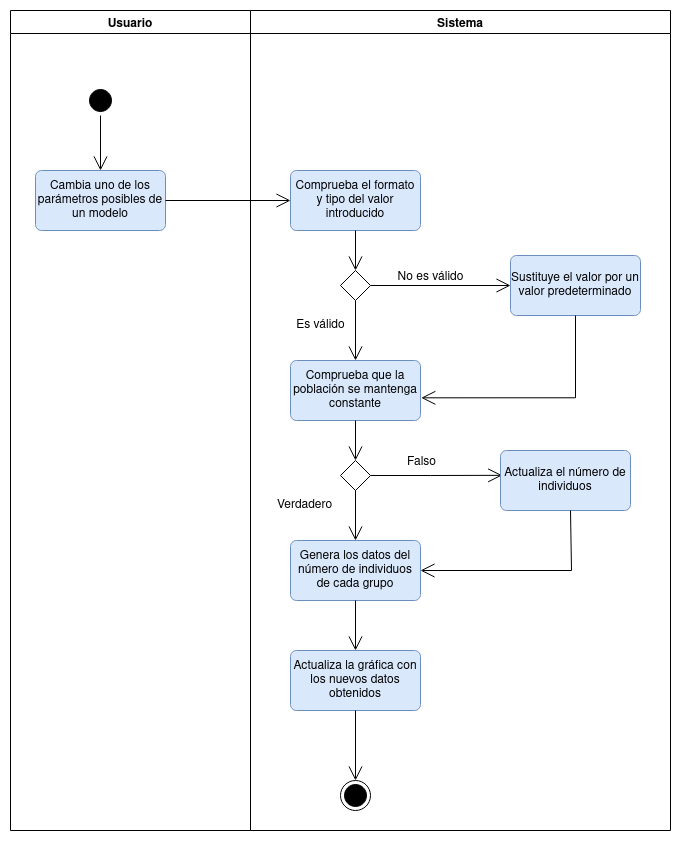
\includegraphics[scale=0.5]{diagrama_actividad-Modificar_parametro.drawio}
\end{center}
\end{figure}

\begin{figure}[!h]
\begin{center}
\caption{Diagrama de actividad del ajuste de datos.}
\label{diag: actividad_ajuste}
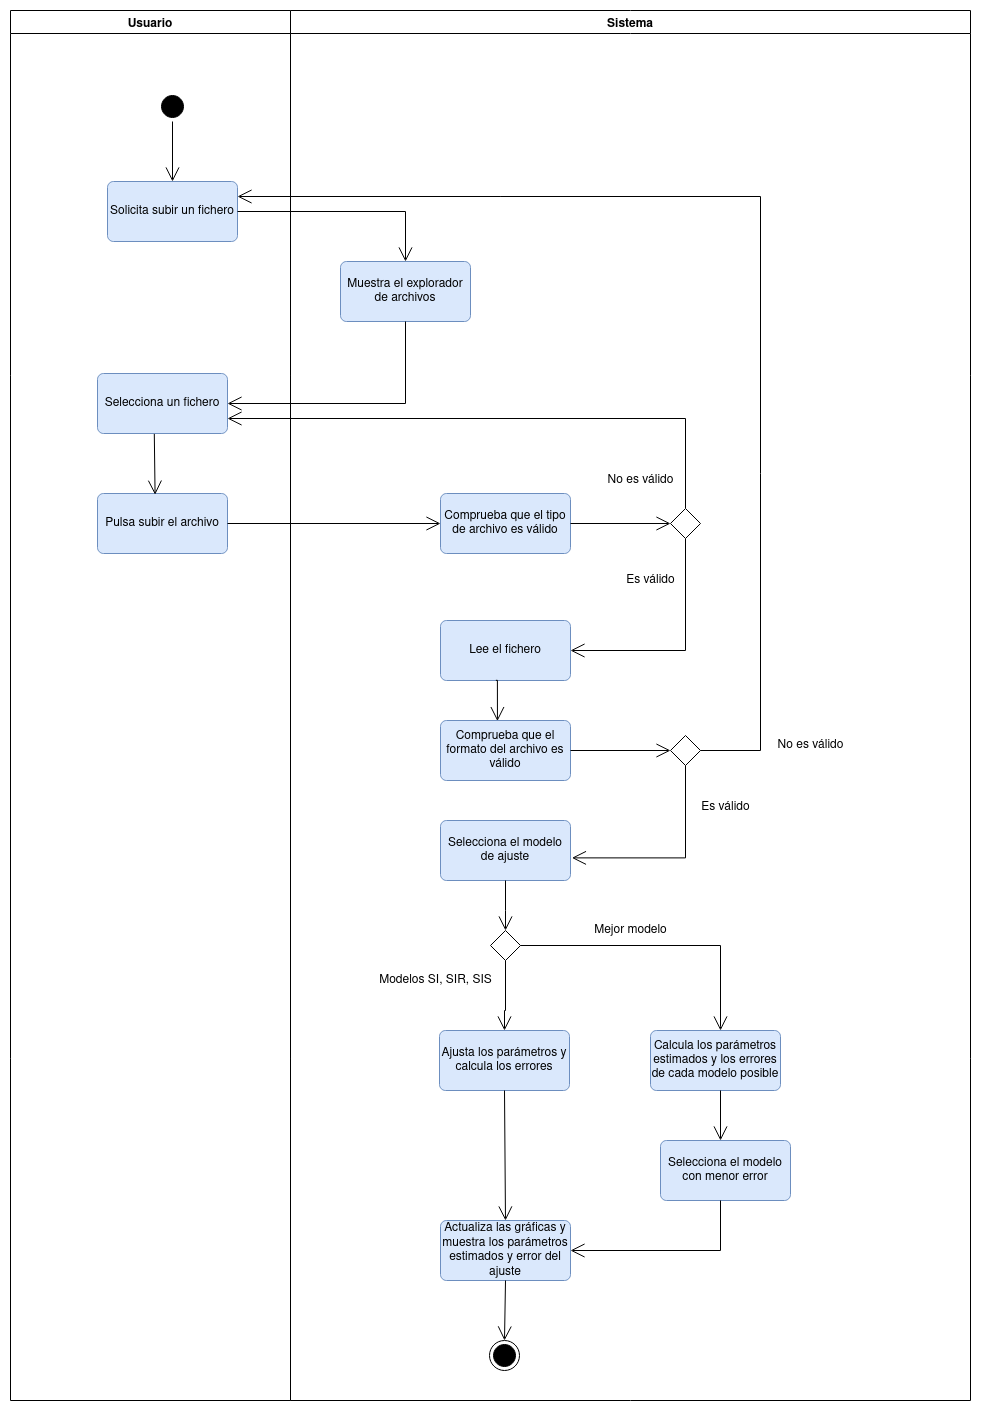
\includegraphics[scale=0.42]{diagrama_actividad-Ajuste_parametros.drawio}
\end{center}
\end{figure}


\section{Pruebas}

A medida que se desarrollaba el proyecto, se han llevado a cabo diversas pruebas de las distintas funcionalidades que se han desarrollado incrementalmente, con el fin de garantizar en todo momento que se disponía de un producto mínimamente viable.

Se han llevado a cabo dos tipos de pruebas:

\begin{itemize}
\item \textbf{Pruebas unitarias:} Tienen como objetivo asegurar el correcto funcionamiento de las funciones creadas de forma independiente de las demás. 
\item \textbf{Pruebas de usuario:} Tratan de simular la interacción entre un usuario y la interfaz del proyecto.
\end{itemize}

\subsection{Pruebas unitarias}

\begin{itemize}
\item \textbf{Preprocesamiento de valores de parámetros.} Se ha probado a introducir diversos valores para los parámetros modificables en los modelos interactivos, con el fin de asegurarnos de que se preprocesan adecuadamente. El comportamiento esperado es sustituir el valor introducido por $0$ en caso de que este sea un carácter o un valor negativo.
\item \textbf{Correcta generación de datos para diversos modelos.} Se han representado gráficamente los datos generados por las funciones de los modelos y contrastando el comportamiento de los datos obtenidos con el descrito en la teoría, asegurando así la correcta generación de los datos de acuerdo a los diversos modelos.
\item \textbf{Subida de ficheros.} Se ha probado a subir ficheros con extensiones permitidas (csv y txt) y comprobado que se han copiado al directorio pertinente para disponer de los ficheros cuando se requiera, así como a subir ficheros con extensiones no permitidas, verificando que se muestra el error correspondiente al no permitirse.
\end{itemize}

\subsection{Pruebas de usuario}

\begin{itemize}
\item \textbf{Prueba de población constante.} Si el usuario introduce valores para las condiciones iniciales ($S_0, I_0$ y $R_0$ si es requerido) tal que su suma no sea $N$ se actualiza el valor de la población de forma que $S_0+I_0+R_0=N$.
\item \textbf{Formato de los valores para parámetros.} Si el usuario introduce un valor de un parámetro con formato incorrecto se sustituye por $0$.
\item \textbf{Condiciones iniciales deben ser números enteros.} Si el usuario introduce un valor no entero positivo se toma como valor real la parte entera del valor introducido por el usuario.
\item \textbf{Subida de fichero inexistente.} Si se trata de subir un fichero al que no se puede acceder o no selecciona ningún fichero antes de pulsar en subir fichero se muestra el error correspondiente.
\item \textbf{Interacción con las gráficas.} Los usuarios pueden hacer zoom, desplazarse y obtener el valor numérico de las representaciones gráficas en cada momento en tiempo real, así como descargar las gráficas generadas.
\end{itemize}

%\clearpage

\section{Diseño de la interfaz de usuario}

Para finalizar el diseño del proyecto, hemos realizado unos prototipos del aspecto aproximado que tendrá la interfaz de la página web en algunas de sus páginas. Se ha tratado de conseguir una interfaz sencilla e intuitiva, que permita al usuario una navegación clara y eficaz por la página web, resultando así cómoda desde el primer momento.

Se han prototipado en concreto las siguientes páginas:

\begin{itemize}
\item \textbf{Home}. La página home o principal de la página web es la primera página que se ve al visitar el sitio. Mostrará el logotipo de la página web y una breve descripción del proyecto. Desde aquí, podemos acceder a todas las demás páginas mediante los menús laterales o el menú de navegación. Esta página puede verse en la figura \ref{wire: home}. Además, los menús en la página serán desplegables. Estos desplegables se ven en el prototipo \ref{wire: home_desplegable}.
\item \textbf{Modelo interactivo}. Se ha diseñado la vista genérica de la página de cualquier modelo interactivo, ya sea discreto o continuo. Se mostrarían en primer lugar las ecuaciones del modelo junto con una explicación del mismo. Bajo esto, se podrían editar los parámetros y encontraríamos las gráficas correspondientes a dichos parámetros. Esta página se muestra en la figura \ref{wire: modelo_interactivo}.
\item \textbf{Ajuste de datos}. También encontramos el prototipo \ref{wire: ajuste}, que muestra el concepto de la página de ajuste de datos. Esta contiene primero una representación gráfica de los datos del fichero subido por el usuario. Después, se muestra un selector para elegir el modelo de ajuste. Finalmente encontramos una gráfica representando los datos junto con el ajuste realizado y la información relativa a valores estimados de parámetros y los errores.
\item \textbf{Ayuda}. Se ha diseñado una página de ayuda con preguntas frecuentes e información de contacto para que, en caso de que los usuarios tuvieran alguna duda sobre el uso de la página, puedan consultarla. Esta página puede verse en el prototipo \ref{wire: ayuda}.
\end{itemize}



\begin{figure}
\begin{center}
\caption{Prototipo de la página home.}
\label{wire: home}
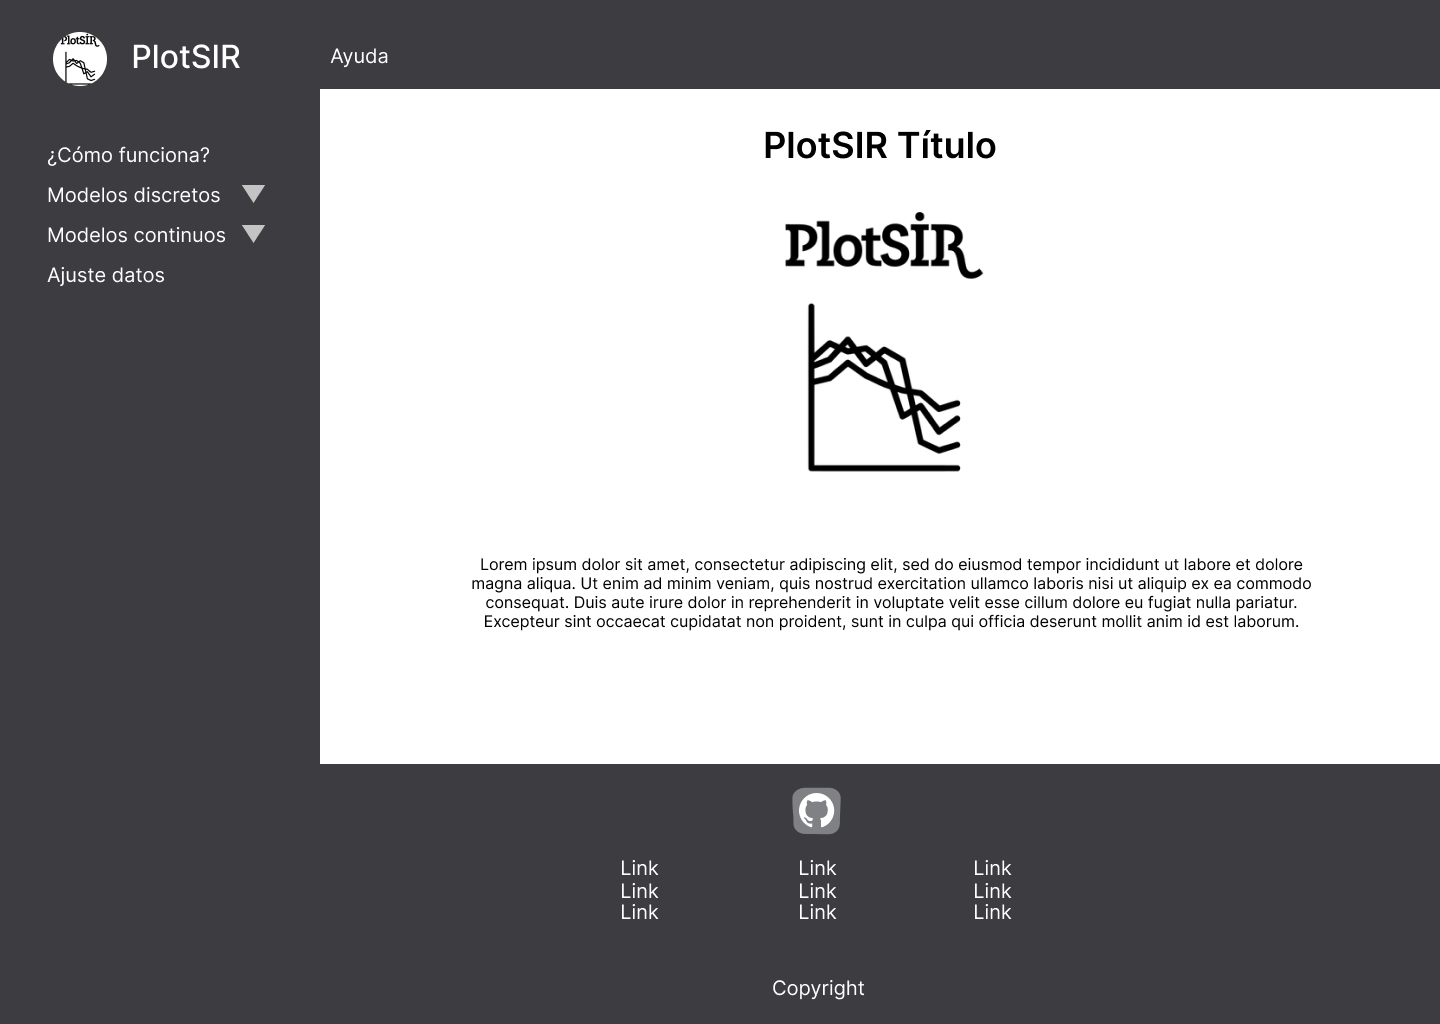
\includegraphics[scale=0.25]{Home}
\end{center}
\end{figure}

\begin{figure}
\begin{center}
\caption{Prototipo de la página home, con desplegable mostrándose.}
\label{wire: home_desplegable}
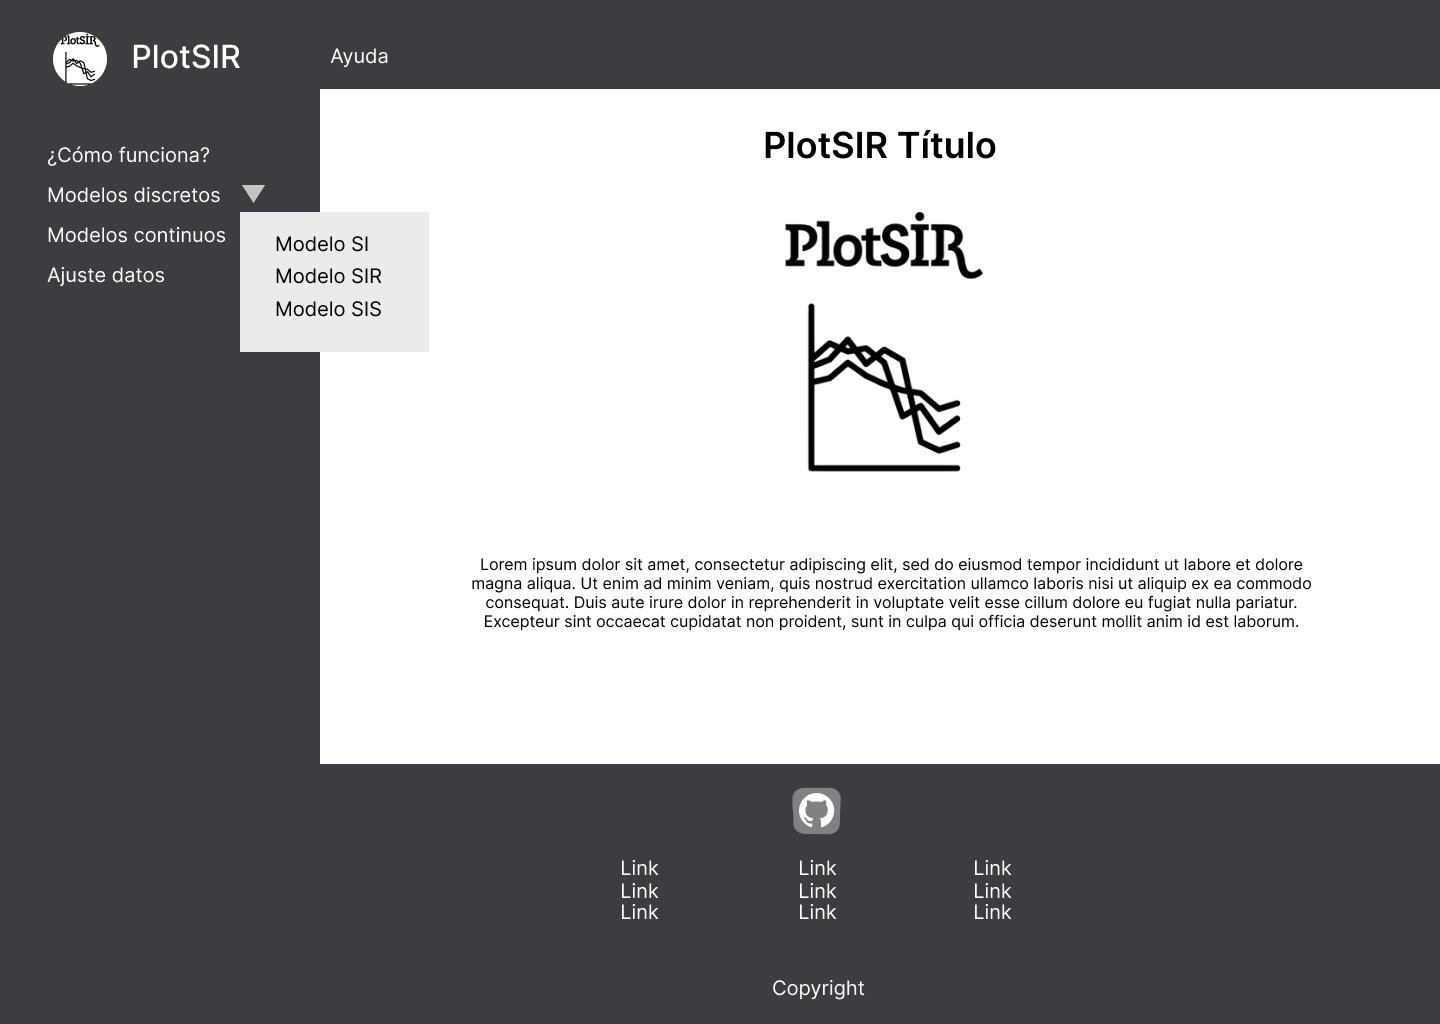
\includegraphics[scale=0.25]{Home_desplegable}
\end{center}
\end{figure}

\begin{figure}
\begin{center}
\caption{Prototipo de la página de un modelo interactivo.}
\label{wire: modelo_interactivo}
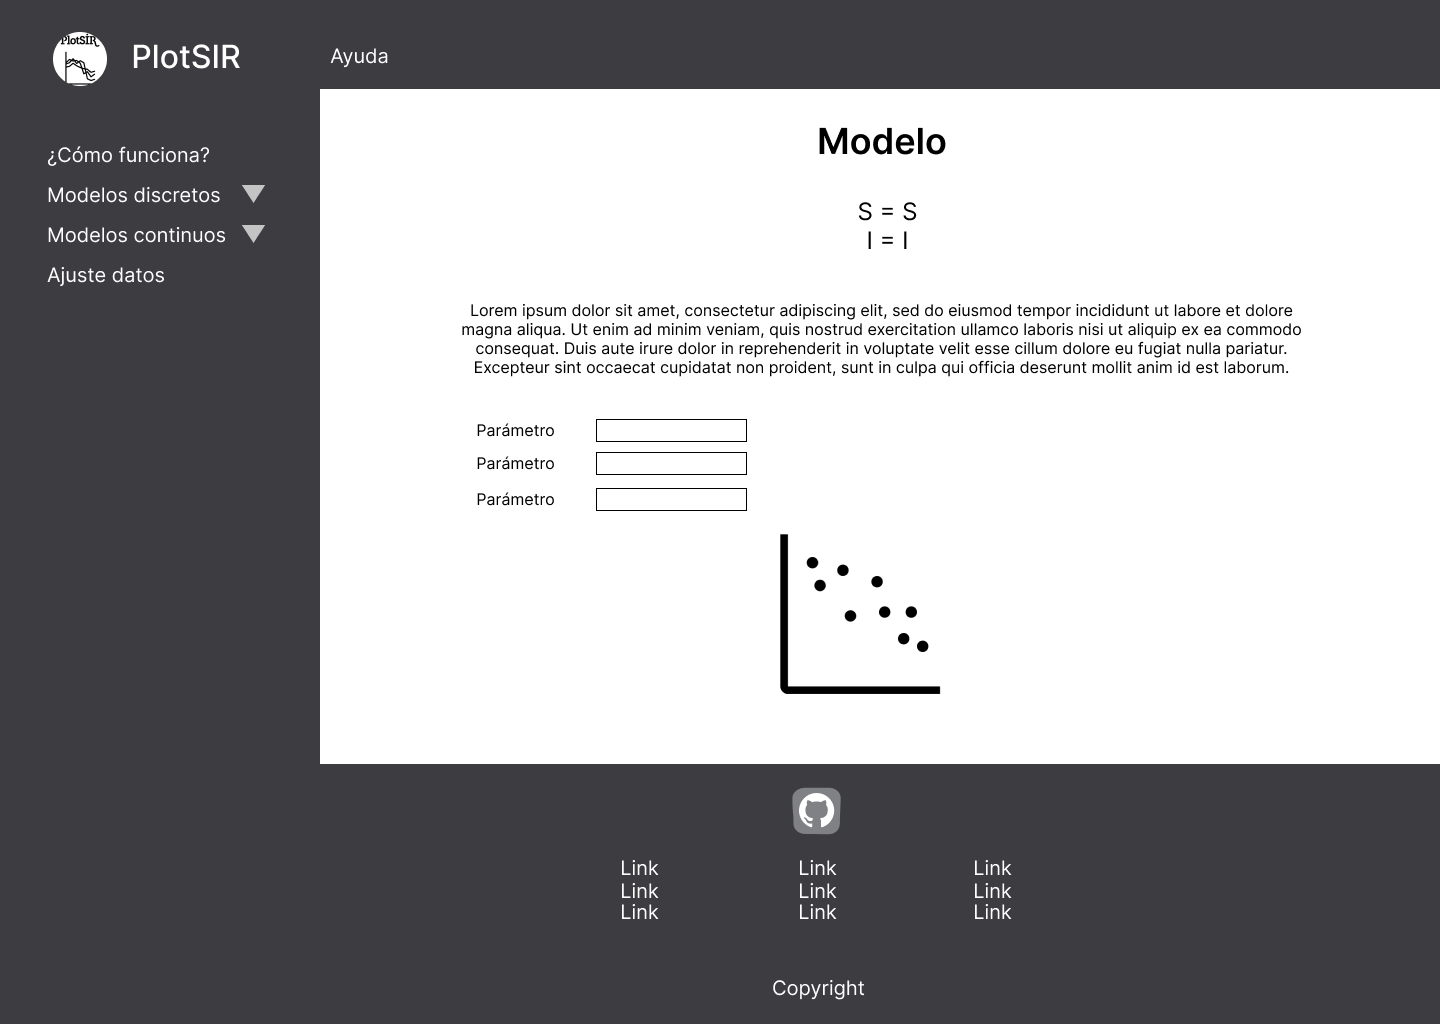
\includegraphics[scale=0.25]{Modelo_interactivo}
\end{center}
\end{figure}

\begin{figure}
\begin{center}
\caption{Prototipo de la página de ajuste de datos subidos desde un fichero.}
\label{wire: ajuste}
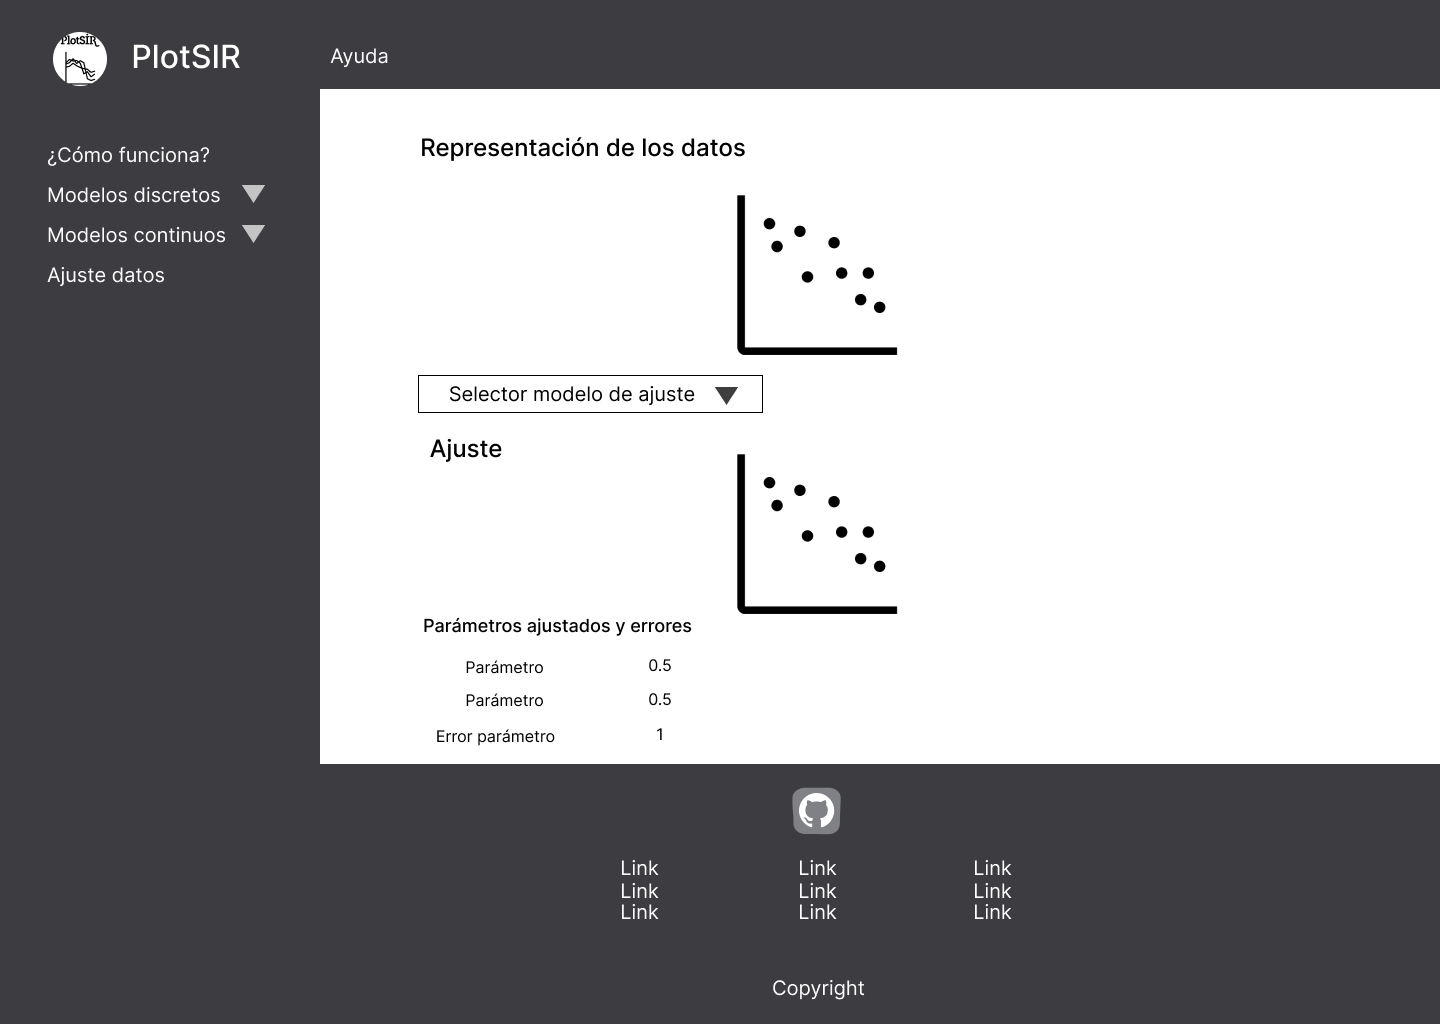
\includegraphics[scale=0.25]{Ajuste_datos}
\end{center}
\end{figure}

\begin{figure}
\begin{center}
\caption{Prototipo de la página de ayuda.}
\label{wire: ayuda}
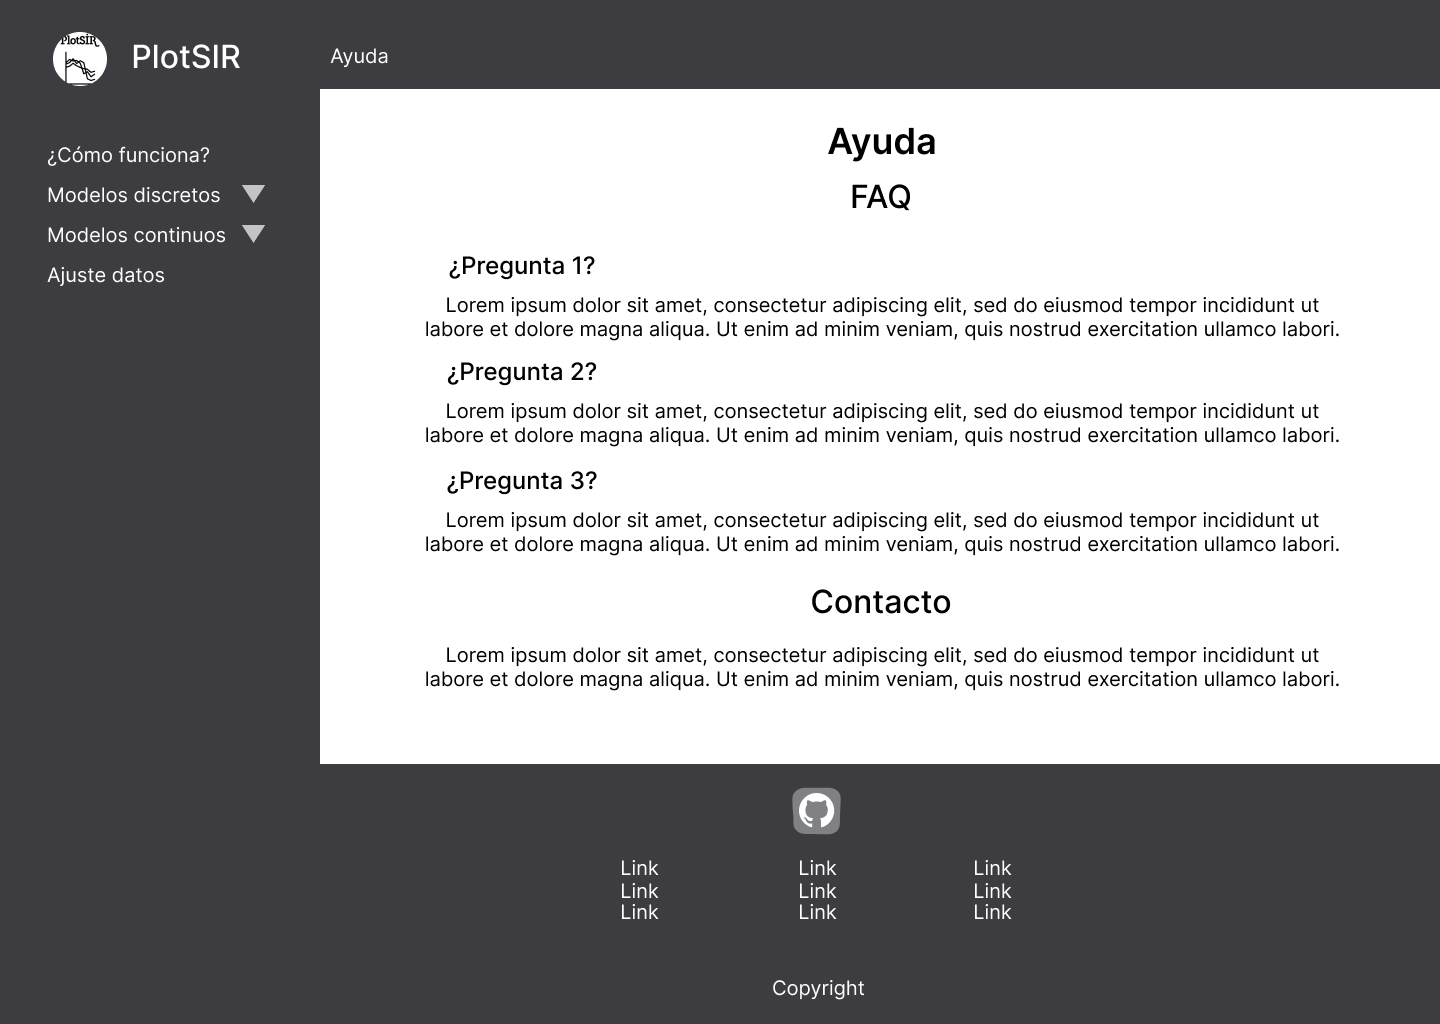
\includegraphics[scale=0.25]{Ayuda}
\end{center}
\end{figure}

\section{Manual de usuario}

\subsection{Descripción del software}

El software consiste en el desarrollo de una página web de objetivo didáctico a la par que práctico, en la que se ofrece información sobre diversos modelos básicos de epidemiología de forma sencilla y clara a cualquier usuario.

De esta forma, el usuario puede aprender sobre varios modelos de epidemiología comprobando interactivamente su comportamiento en tiempo real, y cómo afectan los parámetros de cada uno de ellos a la evolución de los mismos.

Además, se pueden subir ficheros con datos, ya sean generados por el propio usuario o datos reales recogidos y comprobar el resultado de ajustar estos datos a los modelos mencionados, así como elegir el mejor modelo que ajusta dichos datos.

Para acceder a la página web el usuario solo requiere de un dispositivo con un navegador de internet mediante el que acceder a la web, introduciendo la url correspondiente.

\subsection{Comenzando a usar la web}

Una vez introducida la url de la web en el navegador, aparecemos en la página principal de esta, la cual puede verse en la figura \eqref{manual: home}.

\begin{figure}
\begin{center}
\caption{Página home o principal de la web.}
\label{manual: home}
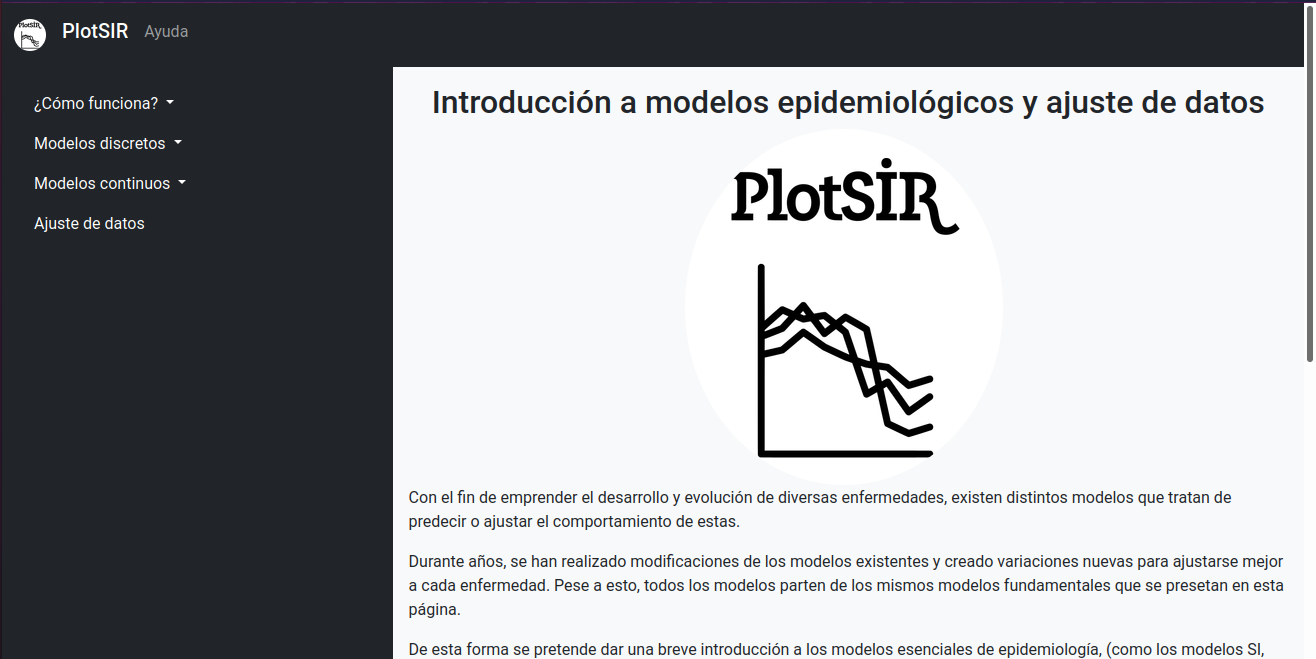
\includegraphics[scale=0.3]{pagina_home}
\end{center}
\end{figure}

Desde esta página podemos acceder a todas las funcionalidades e información de la web desde la barra de navegación y el menú lateral.

Además, la página principal es accesible en cualquier momento. Para volver a ella basta clicar en el logo de la esquina superior izquierda o el nombre de la página situado a su lado.

Asimismo, en la barra de navegación, situado al lado del título de la página encontramos el enlace a la ayuda de la misma. En esta página encontramos dos secciones: preguntas frecuentes, que puede verse en la imagen \ref{manual: ayuda1}, y contacto, que se muestra en la figura \ref{manual: ayuda2}, para recibir asistencia personalizada o sugerir mejoras a la página web.

\begin{figure}
\begin{center}
\caption{Página de ayuda, sección de preguntas frecuentes.}
\label{manual: ayuda1}
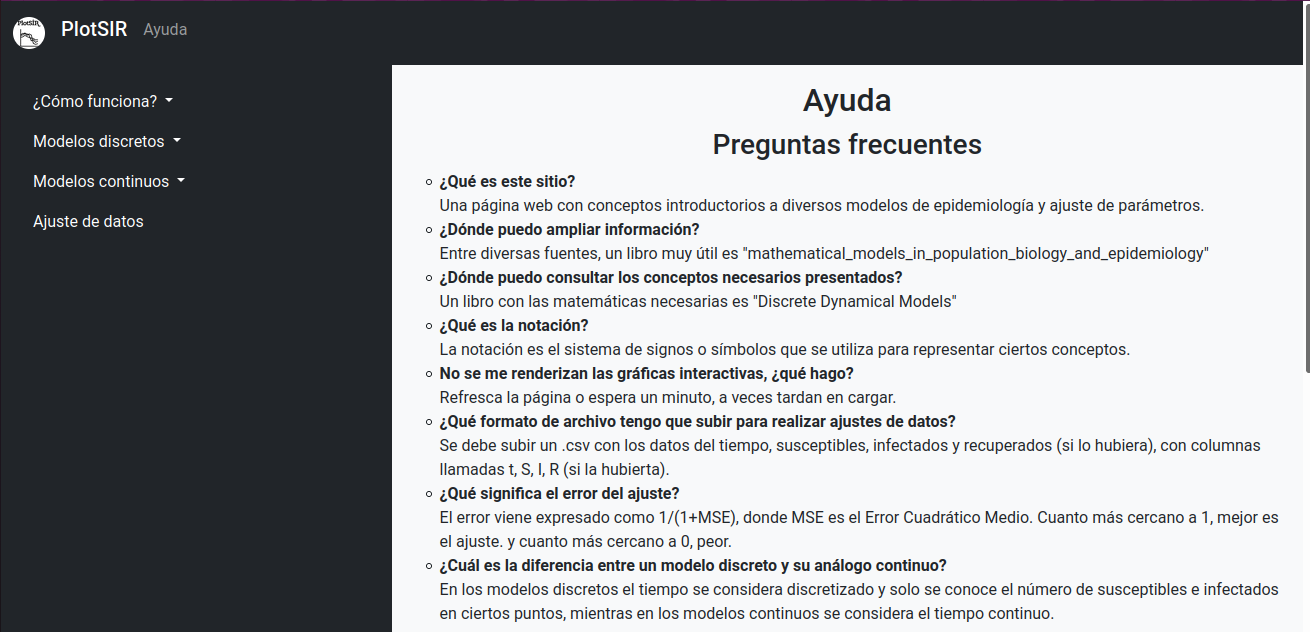
\includegraphics[scale=0.3]{pagina_ayuda}
\end{center}
\end{figure}

\begin{figure}
\begin{center}
\caption{Página de ayuda, sección de contacto.}
\label{manual: ayuda2}
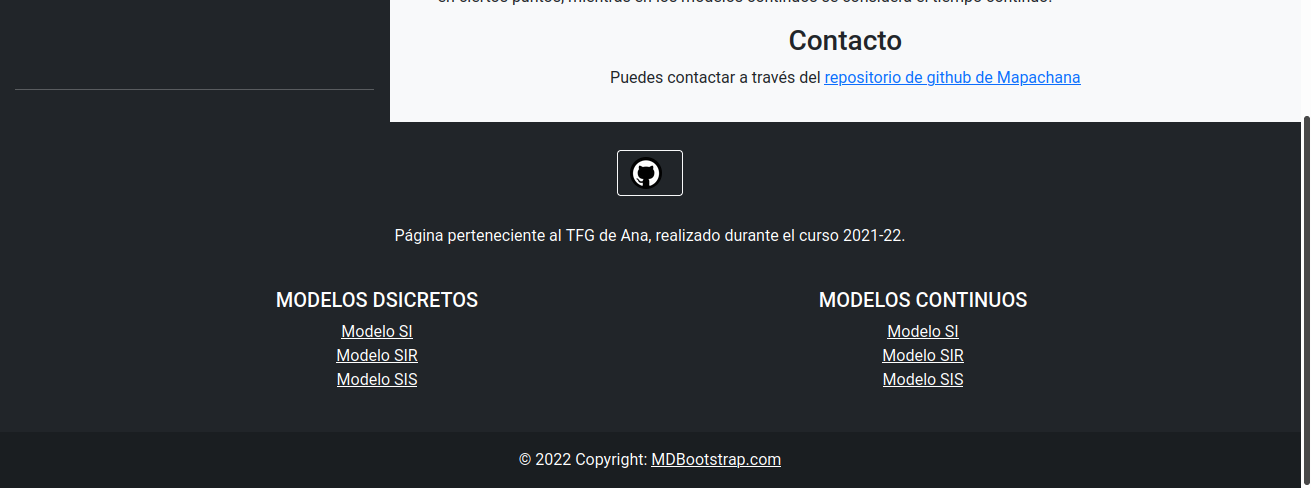
\includegraphics[scale=0.3]{pagina_ayuda2}
\end{center}
\end{figure}

También puede accederse a la página de ayuda desde el menú lateral, clicando en \verb|¿Cómo funciona?| para mostrar las opciones del desplegable y luego en ayuda. Aparte, en \verb|notación| hay un resumen de la notación usada en toda la página web, haciendo fácil consultarla en cualquier momento. El apartado de notación se muestra en la figura \ref{manual: notacion}.

\begin{figure}
\begin{center}
\caption{Página de notación.}
\label{manual: notacion}
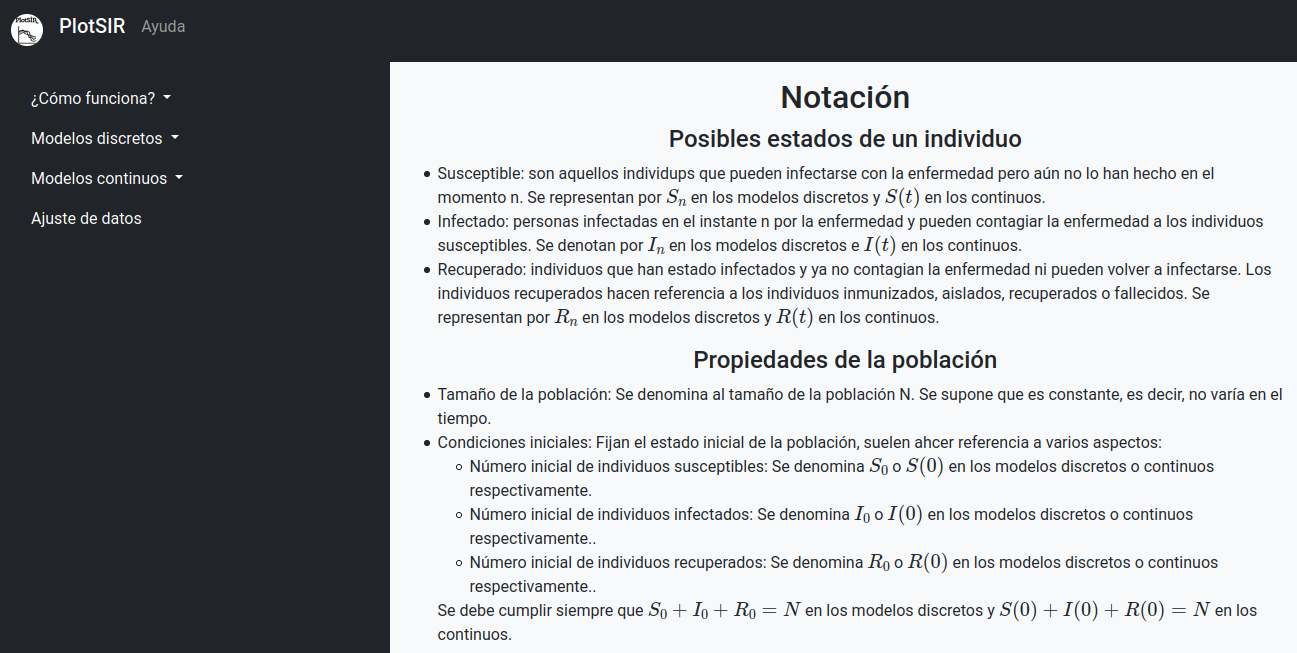
\includegraphics[scale=0.3]{pagina_notacion}
\end{center}
\end{figure}

Finalmente, las distintas funcionalidades de la página se encuentran en el menú lateral. Estas funcionalidades se explican a continuación.

\subsection{Funcionalidades}

\subsubsection{Modificación de parámetros de los modelos interactivos}

En el menú lateral encontramos dos menús desplegables, llamados \verb|Modelos| \verb|discretos| y \verb|Modelos Continuos|. Al pulsar sobre cualquiera de ellos se muestran tres enlaces, a los modelos SI, SIR y SIS, como se ve en la figura \ref{manual: desplegable}. Al seleccionar cualquiera de ellos llegamos a la página de dicho modelo.

\begin{figure}
\begin{center}
\caption{Desplegable de modelos discretos desplegado.}
\label{manual: desplegable}
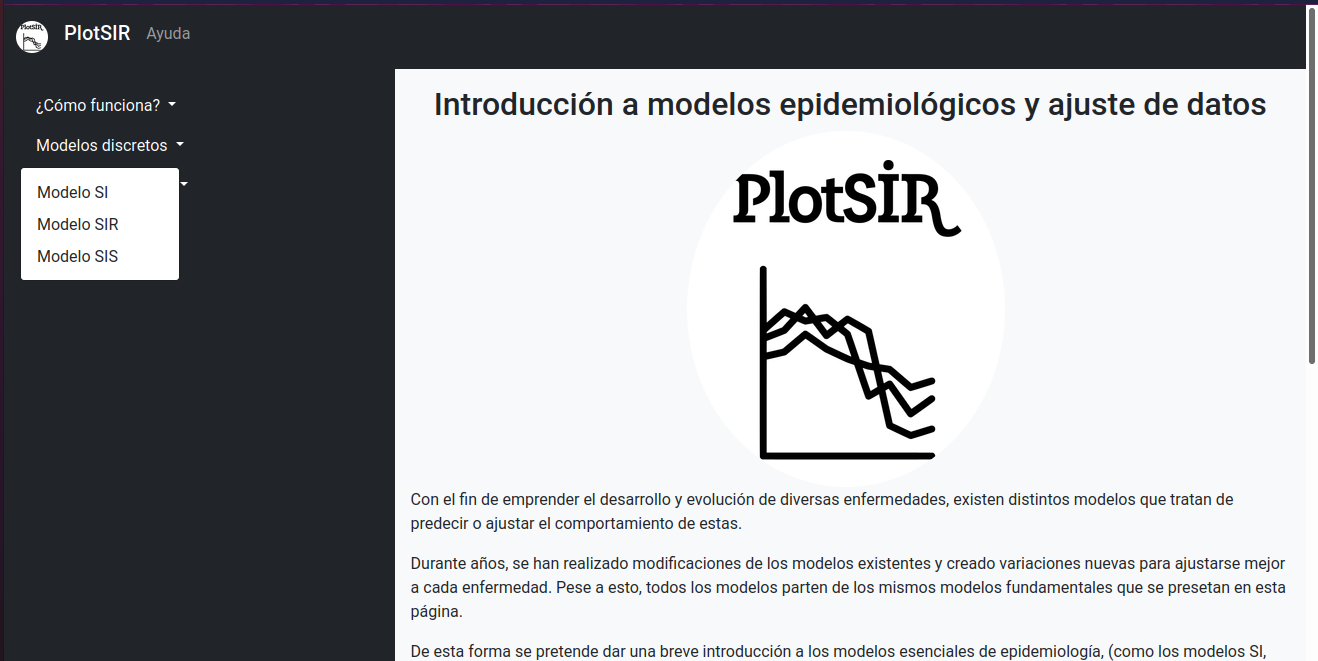
\includegraphics[scale=0.3]{pagina_desplegable}
\end{center}
\end{figure}

En las páginas de los modelos podemos distinguir varias partes principales:

\begin{itemize}
\item Al comienzo de la página de cada modelo se explica la teoría y ecuaciones correspondientes a dicho modelo. Por ejemplo, para el modelo SI discreto se puede ver la explicación teórica en la figura \ref{manual: modeloSI1}.
\item A continuación se muestran los parámetros del modelo, que el usuario puede modificar con el fin de ver cómo varía el comportamiento del modelo que se está estudiando. En el modelo SI por ejemplo se pueden modificar los modelos que se ven en la imagen \ref{manual: modeloSI2}.
\item Finalmente, se muestran una serie de gráficas que ilustran el comportamiento del modelo con los parámetros dados. La primera es una funcion de cada grupo de individuos dependiendo explícitamente del tiempo, se puede ver en la gráfica \ref{manual: modeloSI2}, mientras el resto son funciones implícitas del tiempo, se muestra en la figura \ref{manual: modeloSI3}.
\end{itemize}

\begin{figure}
\begin{center}
\caption{Página del modelo SI, explicación teórica.}
\label{manual: modeloSI1}
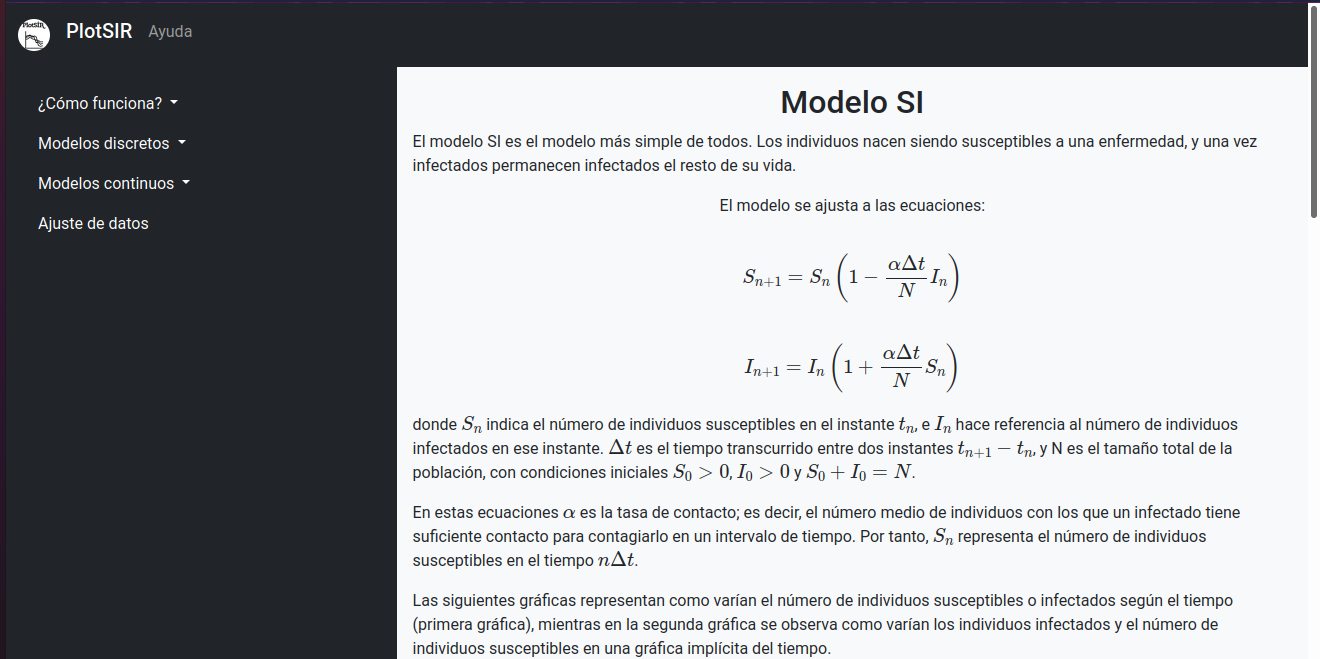
\includegraphics[scale=0.3]{pagina_modeloSI}
\end{center}
\end{figure}

\begin{figure}
\begin{center}
\caption{Página del modelo SI, campos para la modificación de parámetros y gráfica explícita del tiempo.}
\label{manual: modeloSI2}
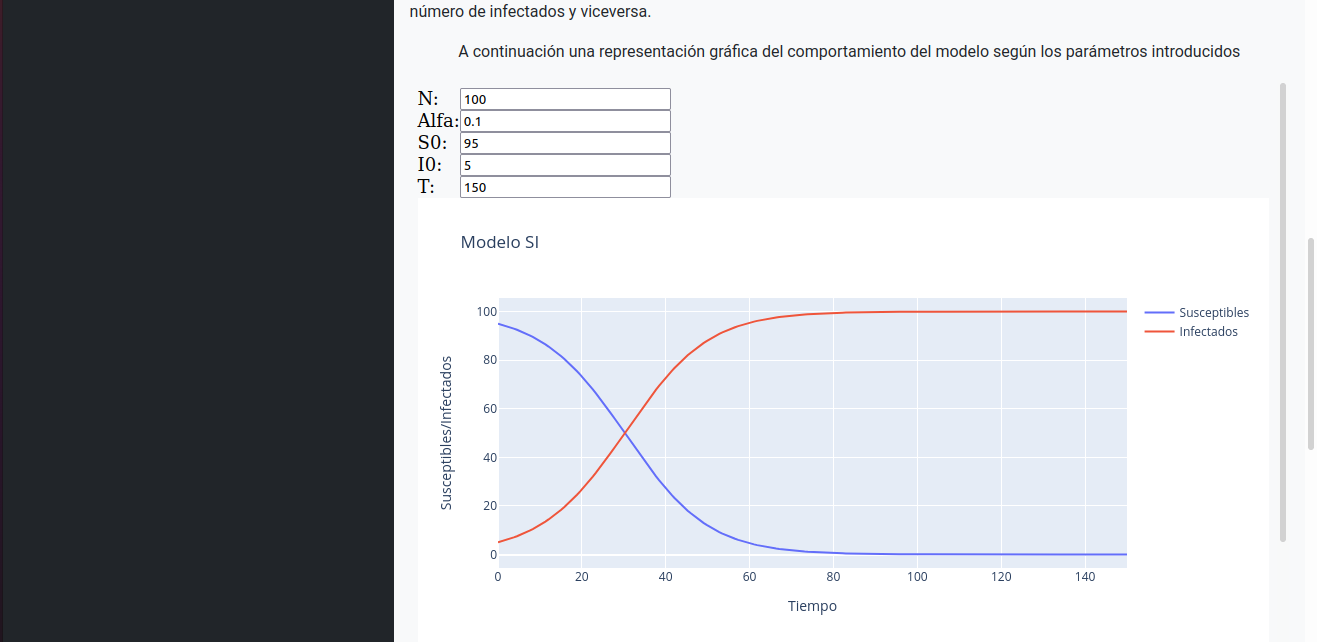
\includegraphics[scale=0.3]{pagina_modeloSI2}
\end{center}
\end{figure}

\begin{figure}
\begin{center}
\caption{Página del modelo SI, gráfica implícita del tiempo.}
\label{manual: modeloSI3}
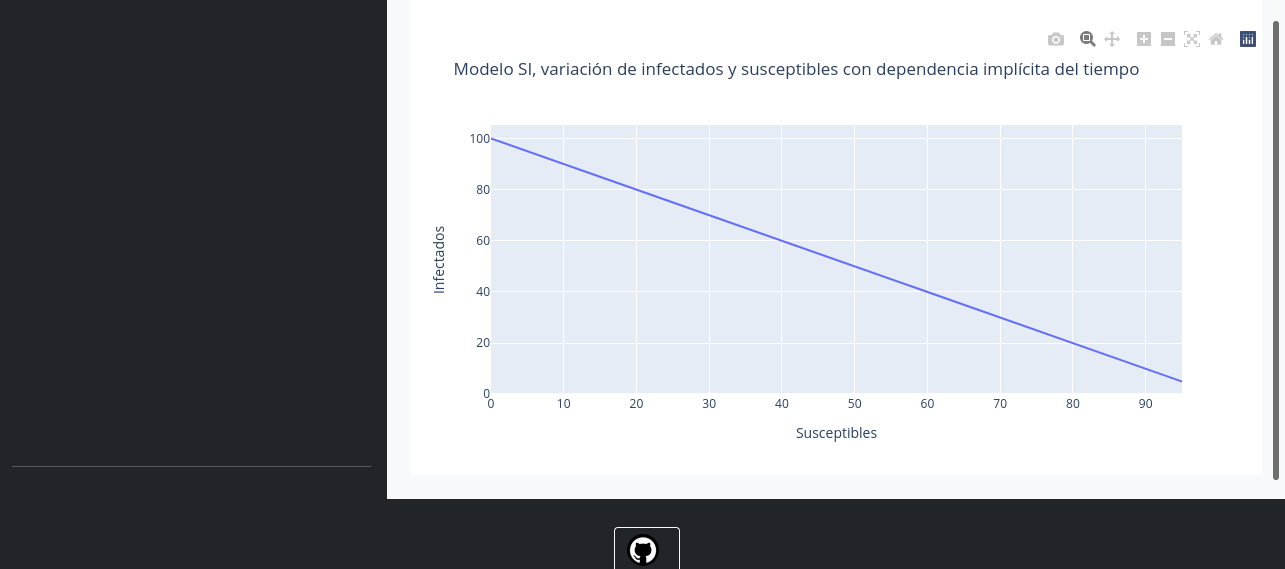
\includegraphics[scale=0.3]{pagina_modeloSI3}
\end{center}
\end{figure}

\subsection{Ajuste de datos}

También es posible subir un fichero en formato \verb|csv| con datos para ajustar con alguno de los modelos disponibles.

Es importante que el fichero a subir tenga como mínimo dos filas y tres columnas llamadas \verb|t|, \verb|S| e \verb|I|, siendo estas el tiempo, los individuos susceptibles en ese tiempo y los individuos infectados en ese tiempo, respectivamente. Adicionalmente, se podría tener una cuarta columna \verb|R| con los recuperados en ese tiempo.

Un ejemplo de un fichero válido sería \verb|fichero_ejemplo.csv| conteniendo:

\begin{verbatim}
t,S,I,R
2003,97.01665754023489,3.377399973205731,-3.816768927775707
2004,102.24543170326915,3.341582397679812,-1.2931795115592053
2005,104.19872670845312,6.0049071497214,-3.2175059735520164
2006,99.79707480976897,10.796475445761393,0.6508408522616295
2007,99.993286104437,3.8927305934099175,0.6722548513086043
\end{verbatim}

Para subir el fichero en la página \ref{manual: ajuste1} seleccionamos \verb|Examinar|, de forma que se abre el navegador de archivos y podemos seleccionar nuestro fichero de datos. Una vez seleccionado pulsamos \verb|Upload| y cargamos el archivo.

\begin{figure}
\begin{center}
\caption{Página de ajuste de datos. Subida de fichero.}
\label{manual: ajuste1}
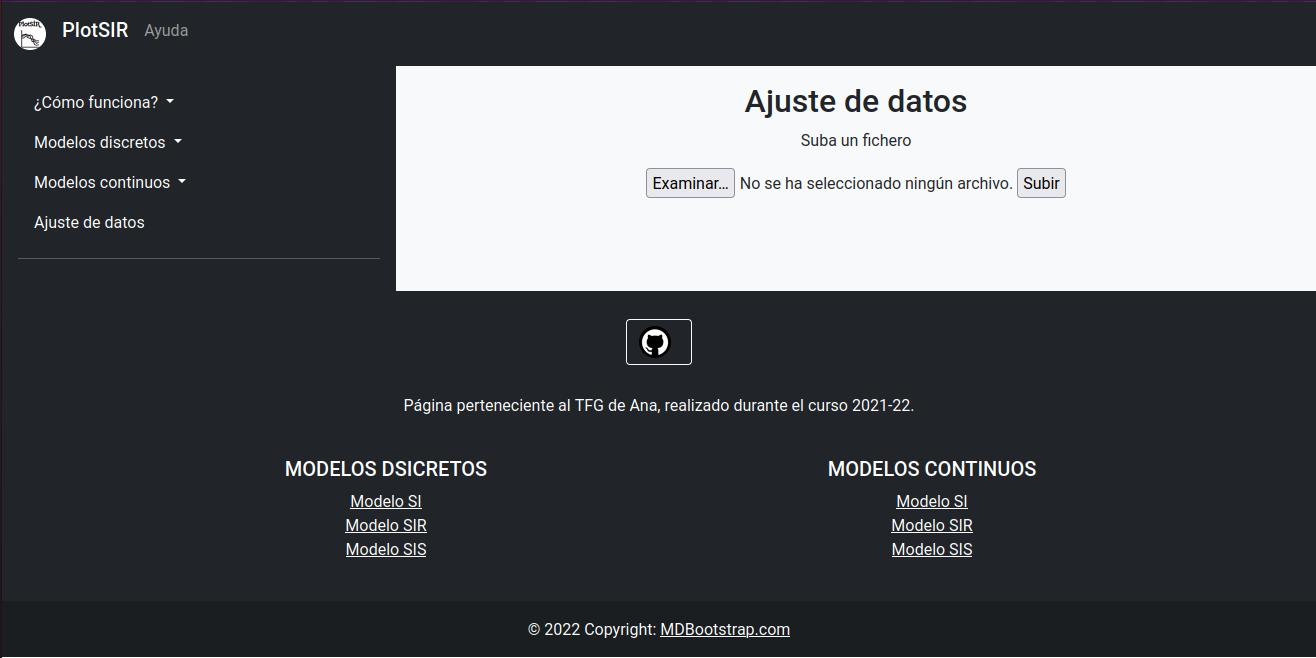
\includegraphics[scale=0.3]{pagina_ajuste}
\end{center}
\end{figure}

\begin{figure}
\begin{center}
\caption{Página de ajuste de datos. Gráfica de representación de los datos del fichero.}
\label{manual: ajuste2}
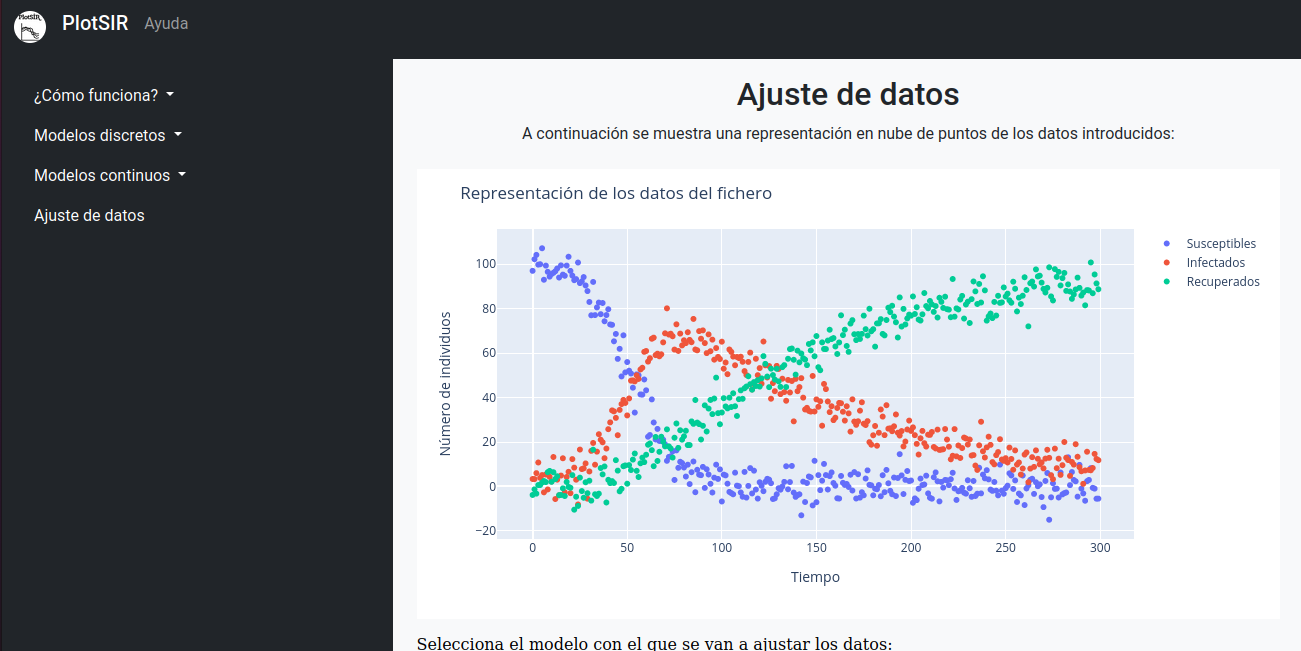
\includegraphics[scale=0.3]{pagina_ajuste2}
\end{center}
\end{figure}

Una vez cargado el fichero se nos muestra una gráfica con los datos del fichero representados, como se ve en la figura \ref{manual: ajuste2}. A continuación, se muestra un desplegable para elegir el modelo con el que se van a intentar ajustar los datos. Las opciones de este son:

\begin{itemize}
\item \textbf{Modelo SI}. Ajusta un modelo SI a los datos.
\item \textbf{Modelo SIR}. Ajusta un modelo SIR a los datos.
\item \textbf{Modelo SIS}. Ajusta un modelo SIS a los datos.
\item \textbf{Mejor modelo}. El sistema decide cuál es el modelo que mejor se ajusta a los datos en base a los errores obtenidos y lo muestra. Realiza el ajuste con dicho modelo.
\end{itemize}

Además, se muestra una gráfica donde se representan los datos y el ajuste obtenido. Este desplegable y la gráfica representando el ajuste se pueden ver en la figura \ref{manual: ajuste3}.

\begin{figure}
\begin{center}
\caption{Página de ajuste de datos. Desplegable y gráfica con el ajuste.}
\label{manual: ajuste3}
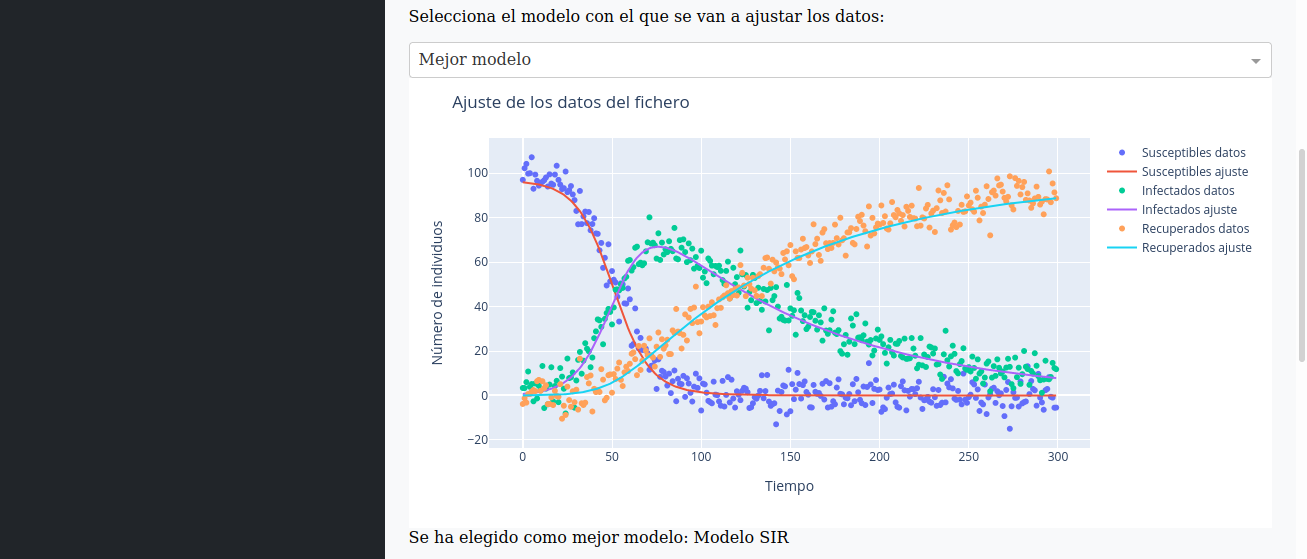
\includegraphics[scale=0.3]{pagina_ajuste3}
\end{center}
\end{figure}

Bajo ella, se muestran las estimaciones de los parámetros de acuerdo al modelo seleccionado y los errores correspondientes. En caso de que la opción para el ajuste haya sido \verb|Mejor modelo| se muestra también el modelo elegido. Estas estimaciones se pueden ver en la figura \ref{manual: ajuste4}. Los valores que se muestran tienen solo 6 cifras decimales por motivos de formato y visualización.

\begin{figure}
\begin{center}
\caption{Página de ajuste de datos. Estimaciones de parámetros y errores.}
\label{manual: ajuste4}

\includegraphics[scale=0.3]{pagina_ajuste4}
\end{center}
\end{figure}


\subsection{Instalación del backend}

Para lanzar la página web de una manera cómoda, rápida y simple, hay varias opciones:

La primera opción consiste en acceder al \href{https://github.com/Mapachana/TFG}{repositorio de Github}\footnote{El enlace es \href{https://github.com/Mapachana/TFG}{https://github.com/Mapachana/TFG}}, descargarlo, colocarnos en la carpeta \verb|codigo/web_plotsir| y ejecutar los comandos:

\begin{verbatim}
make install_deps
make -j2
\end{verbatim}

Una vez hecho esto, ya podemos acceder a la url \verb|localhost:5000| en el navegador.

Como alternativa, se ha creado un contenedor docker actualizado con todas las dependencias necesarias para el funcionamiento de la misma.

De esta manera, basta con ejecutar el contenedor docker, accesible en Docker Hub, descargarlo y ejecutarlo. El contenedor puede obtenerse \href{https://hub.docker.com/repository/docker/mapachana/plotsir}{aquí}\footnote{El enlace es \href{https://hub.docker.com/repository/docker/mapachana/plotsir}{https://hub.docker.com/repository/docker/mapachana/plotsir}}.

Para obtener y lanzar la imagen debe abrirse una terminal y ejecutar los siguientes comandos:

\begin{verbatim}
docker pull mapachana/plotsir:latest
docker run -t -p 5000:5000 -p 8050:8050  mapachana/plotsir:latest
\end{verbatim}

Tras esto accedemos a la url \verb|localhost:5000| en nuestro navegador.


\section{Datos reales}

Una vez estudiados los modelos teóricos y terminada la implementación vamos a realizar el ajuste de varios modelos aplicado a datos reales de enfermedades. De esta forma, podemos comprobar si los modelos estudiados sirven para ajustar los datos de algunas enfermedades, ayudando también así a la comprensión de la evolución de estas.

A lo largo de esta sección, los valores que se presentan se muestran con una precisión de $6$ cifras decimales por motivos de formato y visualización.

\section{El VIH en Baleares}

El VIH (Virus de Inmunodeficiencia Humana) es un virus que ataca al sistema inmunitario del cuerpo. Si no se trata, puede causar SIDA. Actualmente no hay ninguna cura efectiva contra el VIH, por lo que una vez que se contrae, se tiene de por vida.

El VIH provino de una especie de chimpancé de África, desde la que se propagó primero por dicho continente, y se estima que lleva en Estados Unidos desde finales de los años 70.

Dado que es una enfermedad para la que una vez infectado siempre se es portador, se tiene que sigue un modelo SI.

El conjunto de datos escogido contiene los datos de los reportes de nuevos infectados por VIH en Baleares anualmente desde 2003 hasta 2019. La fuente utilizada para dichos datos es \cite{datos_vih}.

En el informe se proporcionan los nuevos casos detectados, luego los datos con los que vamos a trabajar son la suma acumulada de estos casos nuevos. Esto se debe a que el modelo considera los casos activos, no solo los nuevos. Por tanto, tenemos que los casos activos son los nuevos más todos los que había antes.

Además, para que el modelo funcione bien el número total de individuos consideramos es el número de individuos estudiados, en este caso $N=2704$.

Teniendo esto en cuenta, generamos un fichero csv con el formato de la página web.

Primeramente, observamos la representación de los datos en la figura \ref{datos_vih}. Vemos que el número de individuos susceptibles va descendiendo, así como el de infectados creciendo en términos globales. Pese a esto, en ciertas partes de la gráfica se aprecia una leve curvatura, donde los datos de susceptibles pasan de ser cóncavos a convexos y los datos de infectados de convexo a cóncavo.

\begin{figure}
\begin{center}
\caption{Representación de los datos del VIH en Baleares.}
\label{datos_vih}
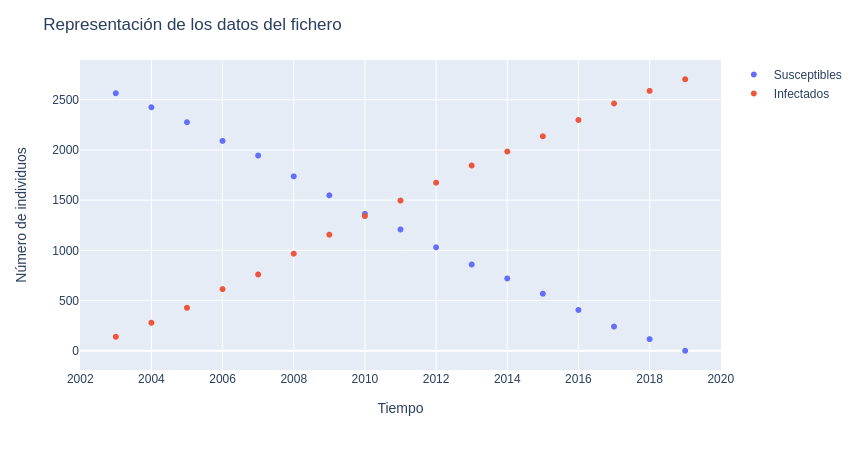
\includegraphics[scale=0.5]{datos_vih}
\end{center}
\end{figure}

Elegimos como modelo de ajuste mejor modelo, donde obtenemos que el mejor modelo según el sistema es, como se comentaba inicialmente, el modelo SI.

La representación gráfica del ajuste se puede ver en la figura \ref{ajuste_vih}. En las curvas del ajuste generado apreciamos con mayor claridad ese cambio de curvatura de cóncavo a convexo y viceversa. 

\begin{figure}
\begin{center}
\caption{Representación del ajuste con el modelo SI a los datos del VIH en Baleares.}
\label{ajuste_vih}
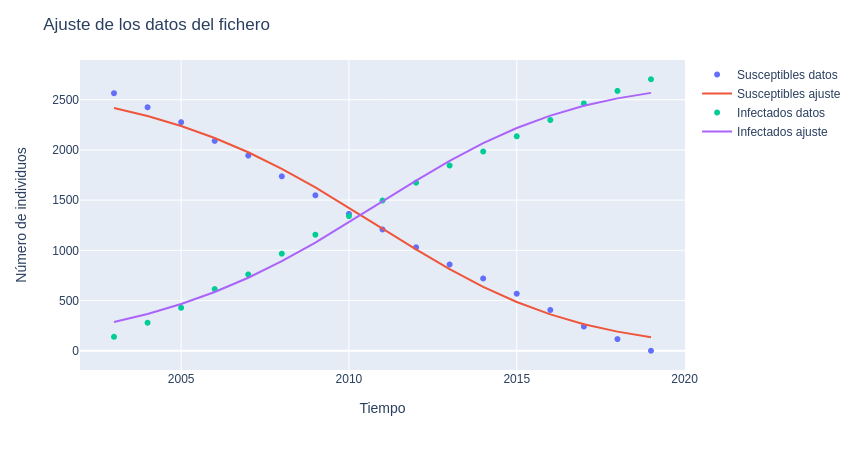
\includegraphics[scale=0.5]{ajuste_vih}
\end{center}
\end{figure}

En  la gráfica \ref{estimacion_vih} se muestra la estimación de los parámetros obtenidos para el ajuste, resultando un $\alpha \approx 0.31$ e $I_0 \approx 287$. Dado que los valores de estos parámetros son razonables y la representación gráfica del ajuste aproxima relativamente bien los datos obtenidos, parece que las infecciones por VIH en Baleares en efecto siguen un modelo SI.

\begin{figure}
\begin{center}
\caption{Estimaciones y errores del ajuste con el modelo SI a los datos del VIH en Baleares.}
\label{estimacion_vih}
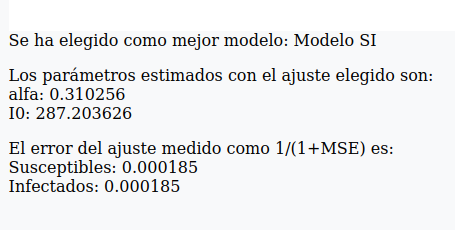
\includegraphics[scale=0.5]{estimacion_vih}
\end{center}
\end{figure}

\section{El Covid-19 en España}

El Covid-19 es una enfermedad respiratoria aguda causada por el virus SARS-CoV-2. Se informó respecto a ella por primera vez en Diciembre de 2019, tras detectarse varios casos en Wuhan. Posteriormente se extendió a otros países, entre los que se encuentra España.

A lo largo de la pandemia del Covid-19 en el mundo se han recopilado una gran cantidad de datos para estudiar esta enfermedad. Para este estudio vamos a usar el conjunto de datos obtenido de \cite{datos_covid}.

En \cite{enrique_amaro} se comprueba que se puede modelar mediante el modelo SIR. Vamos a tratar de ajustarla siguiendo este modelo.

En el fichero csv de los datos hay mucha información, pero realmente solo vamos a usar las columnas \verb|new_cases|, que indica los nuevos casos reportados y \verb|new_deaths|, que informa de las nuevas muertes.

Del fichero nos quedamos con los datos de España y esas dos columnas, que a continuación trataremos, ya que al igual que en el caso anterior, necesitamos trabajar con todos los casos activos y todos los recuperados hasta el momento.

Vamos a ajustar solo el principio de la pandemia, en concreto vamos a ajustar a partir del día de 5 de Marzo de 2020, ya que en los 10 días anteriores no hay datos reportados pese a que aparecen en los datos, y durante los siguientes 170 días, esto es, hasta el 21 de Agosto de 2020, pues es aproximadamente 6 meses, lo que se estima duró lo que se conoce coloquialmente como la primera ola.

Por comodidad, vamos a tratar los datos como indexados en el tiempo, correspondiendo por tanto al 5 de Marzo el índice 0 y al 21 de Agosto el 170.

\begin{figure}
\begin{center}
\caption{Representación de los datos del Covid-19 en España desde el 5 de Marzo hasta el 21 de Agosto de 2020.}
\label{datos_covid}
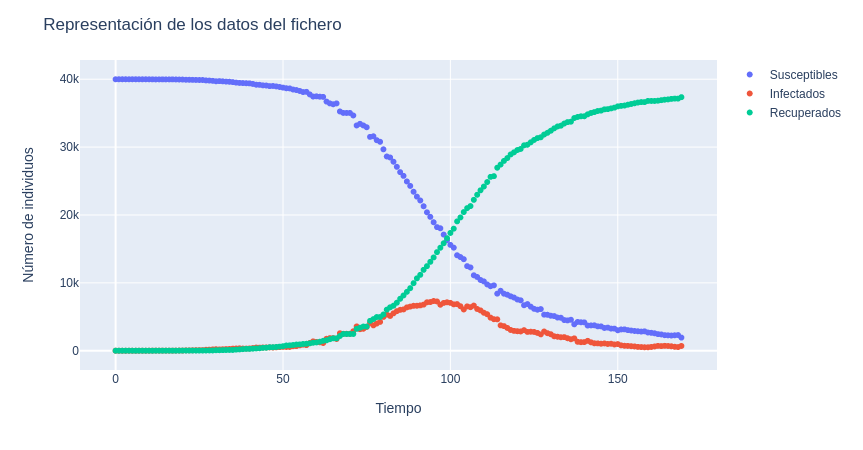
\includegraphics[scale=0.5]{datos_covid}
\end{center}
\end{figure}

Es importante ajustar solamente una ola, pues el modelo SIR considera que tras recuperarse, los individuos no vuelven a ser susceptibles ni a infectarse, pero esto no es así en la realidad. Como el tiempo promedio necesario para volver a ser susceptible a la enfermedad tras recuperarse de esta es mayor que la duración de una ola, este efecto puede ser despreciado. Por tanto, el modelo SIR ajusta solamente las olas de forma independiente. 

Para calcular el número de infectados activos, dado que el Covid-19 al principio de la pandemia tenía una duración aproximada de 10 días, se han considerado todos los nuevos casos reportados desde 10 días atrás hasta ese día como activos.

Asimismo, como recuperados se han considerados los fallecidos y los nuevos infectados de hace más de 10 días atrás, pues ya habrían superado la enfermedad y no podrían volver a infectarse.

\begin{figure}
\begin{center}
\caption{Representación del ajuste con el modelo SIR a los datos del Covid-19 en España desde el 5 de Marzo hasta el 21 de Agosto de 2020.}
\label{ajuste_covid}
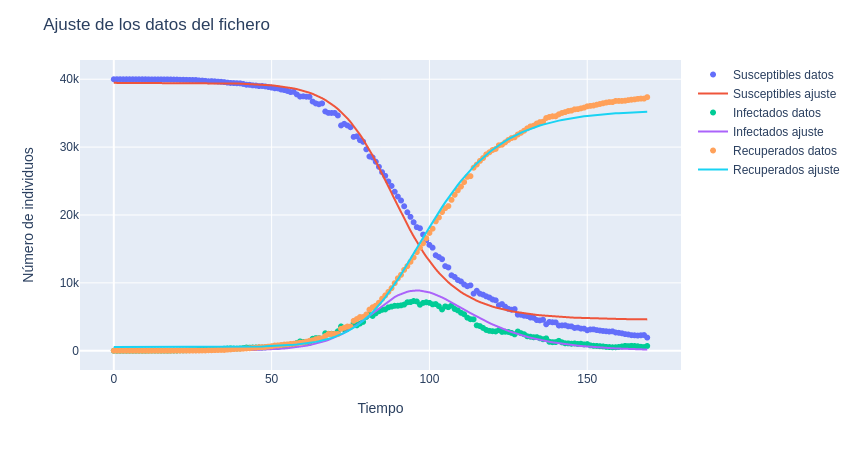
\includegraphics[scale=0.5]{ajuste_covid}
\end{center}
\end{figure}

Además, para que el modelo funcione bien el número total de individuos considerados es el número de individuos estudiados aproximadamente, en este caso $N=40000$.

Teniendo esto en cuenta, generamos un fichero csv con el formato necesario para realizar un ajuste en la página web.

\begin{figure}
\begin{center}
\caption{Estimaciones y errores del ajuste con el modelo SIR a los datos del Covid-19 en España.}
\label{estimacion_covid}
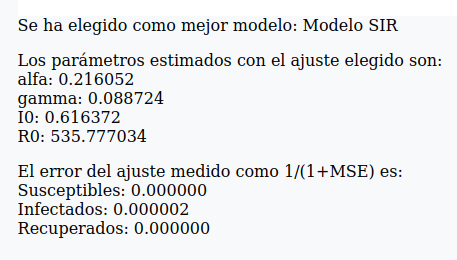
\includegraphics[scale=0.5]{estimacion_covid}
\end{center}
\end{figure}

Al igual que antes, comenzamos observando la representación de los datos en la gráfica \ref{datos_covid}. El número de recuperados siempre es creciente, así como el de susceptibles es siempre decreciente. Llama la atención la forma de los infectados, que primero suben y luego descienden, indicando así el final de la ola.

Elegimos como modelo de ajuste mejor modelo, donde obtenemos que el mejor modelo según el sistema es, como se comentaba inicialmente, el modelo SIR.

La representación gráfica del ajuste se puede ver en la figura \ref{ajuste_covid}. El ajuste parece seguir las tendencias generales de los datos, aunque los infectados quedan ligeramente por encima en el ajuste que en los datos experimentales, así como los recuperados y susceptibles ajustan peor al final, pues cuanto más nos alejamos de la ola en sí, peor es el ajuste al modelo SIR.

En la figura \ref{estimacion_covid} se muestra la estimación de los parámetros obtenidos para el ajuste, resultando un $\alpha \approx 0.21$, $\gamma \approx 0.08$, $I_0 \approx 1$, $R_0 \approx 536$. Dado que los valores de estos parámetros son razonables, salvo quizá por una estimación ligeramente alta de los recuperados iniciales, y la representación gráfica del ajuste aproxima relativamente bien los datos obtenidos, parece que las infecciones por Covid-19 en España en efecto siguen un modelo SIR.













